\chapter{Comparison Between Other Methods}
\label{c:comparision}

\section{Different Feature Point Extraction \& Point Matching Methods}
	% test functions provides in opencv
	% https://docs.opencv.org/3.3.1/d5/d51/group__features2d__main.html
	In this section, we'll discuss how different feature point performs in keyboard defect detection scenario.
	Since the bottleneck of this project is the feature point detection method, we tried some common methods, and below is the observation \& time comparison between different approach.
	\subsection{Experiment Method}
		\subsubsection{Problems}
			We'll discuss the robustness against different kinds of interference this system would encountered in production line.
			The interference most likely happen would be 
			unexpected rotate \& translate when the operator put keyboard on the fixture, 
			LED failure on the main board of keyboard and noise from camera.
		\subsubsection{Testing Methods}
			We'll estimate the robustness by simulate the problems just mentioned. 
			For the testing, we'll first input a reference image and a sample image that copied from reference image, 
			than apply some operations on the sample image to simulate the possible interference on the production line.
			Then we'll apply the image alignment to see when the alignment fails, then discuss the results from different \\
	\subsection{Normal Case}
		This section we'll provide an example of execution without any interference, this case would be the ideal case for the inspection.
		In ideal case, the absolute difference result (\ref{fig:AbsoluteDifferenceResultNormal}) should looks like a plane black image. If there is any misalignment, the absolute difference result would appear radius shaped bright spots.
		In this ideal scenario, every feature point detector were having good results.
		\begin{figure}[H]
			\subfigure[Reference Image]
			{
				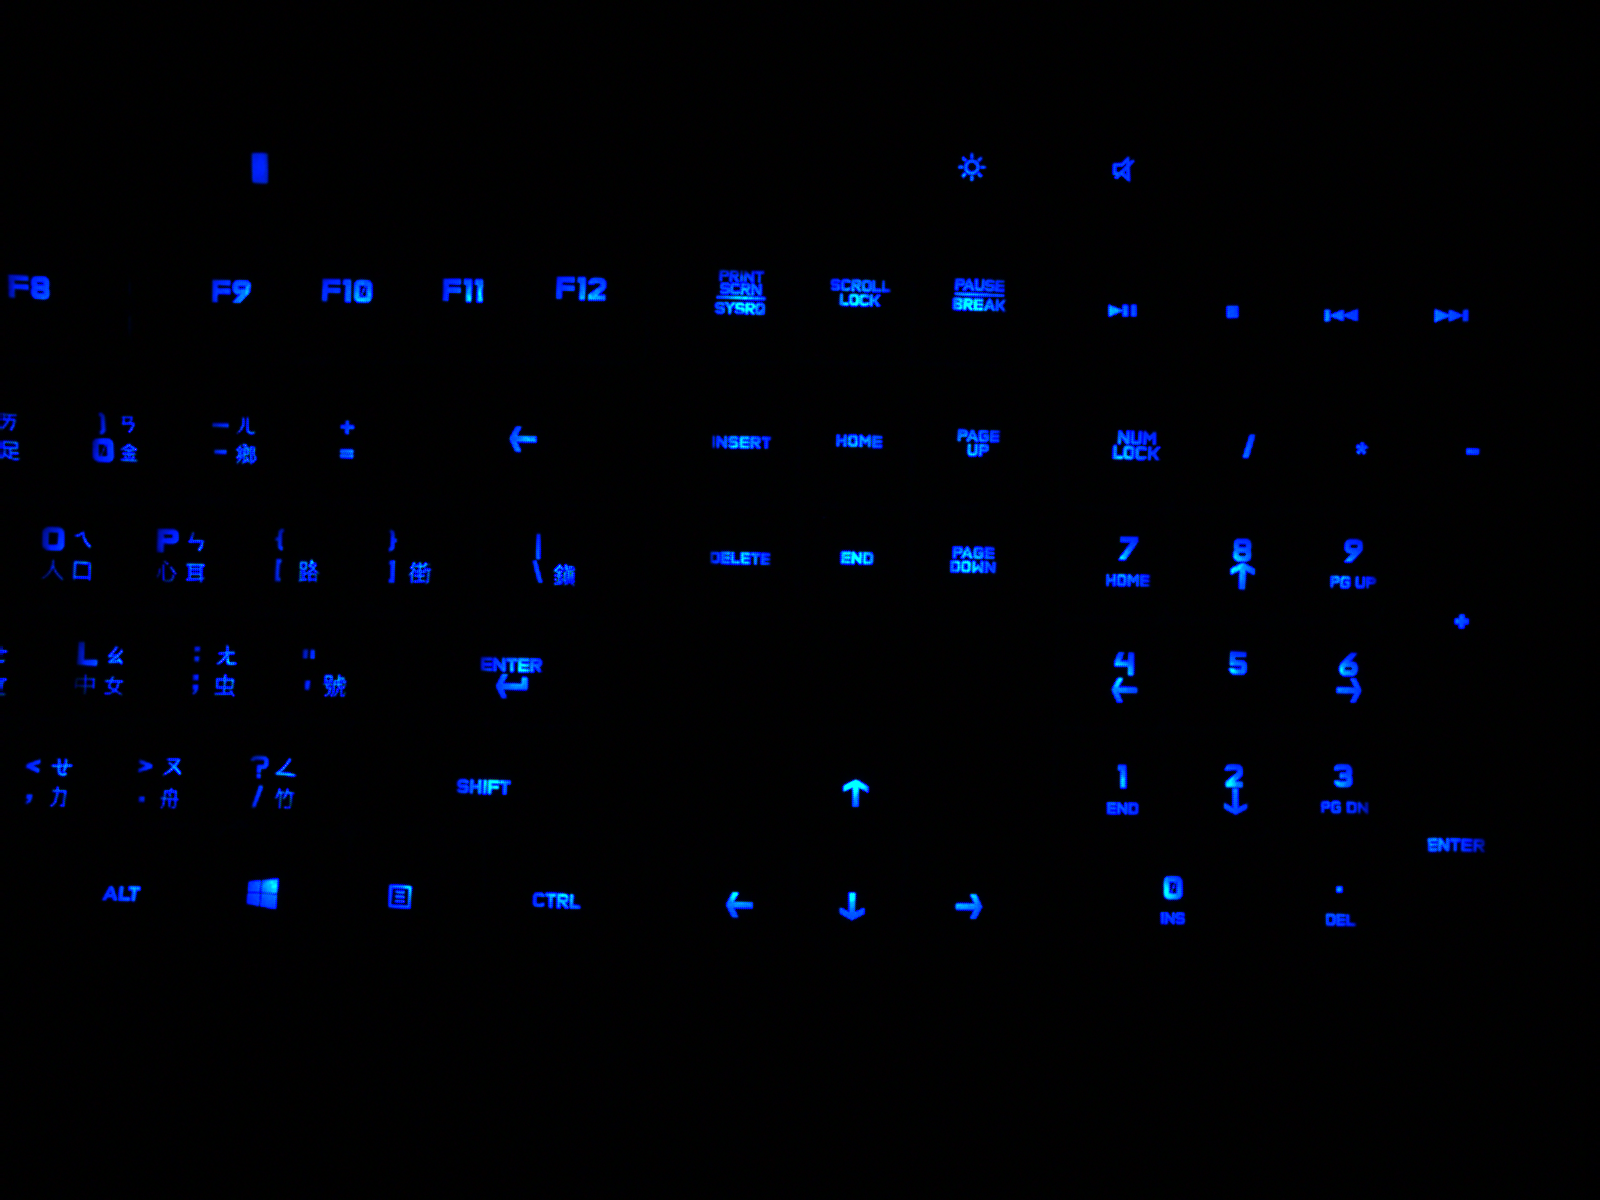
\includegraphics[width=0.5\linewidth]{simulation/normal/input_gold.png}
			}
			\subfigure[Sample Image without Adding Noises \& Distortion]
			{
				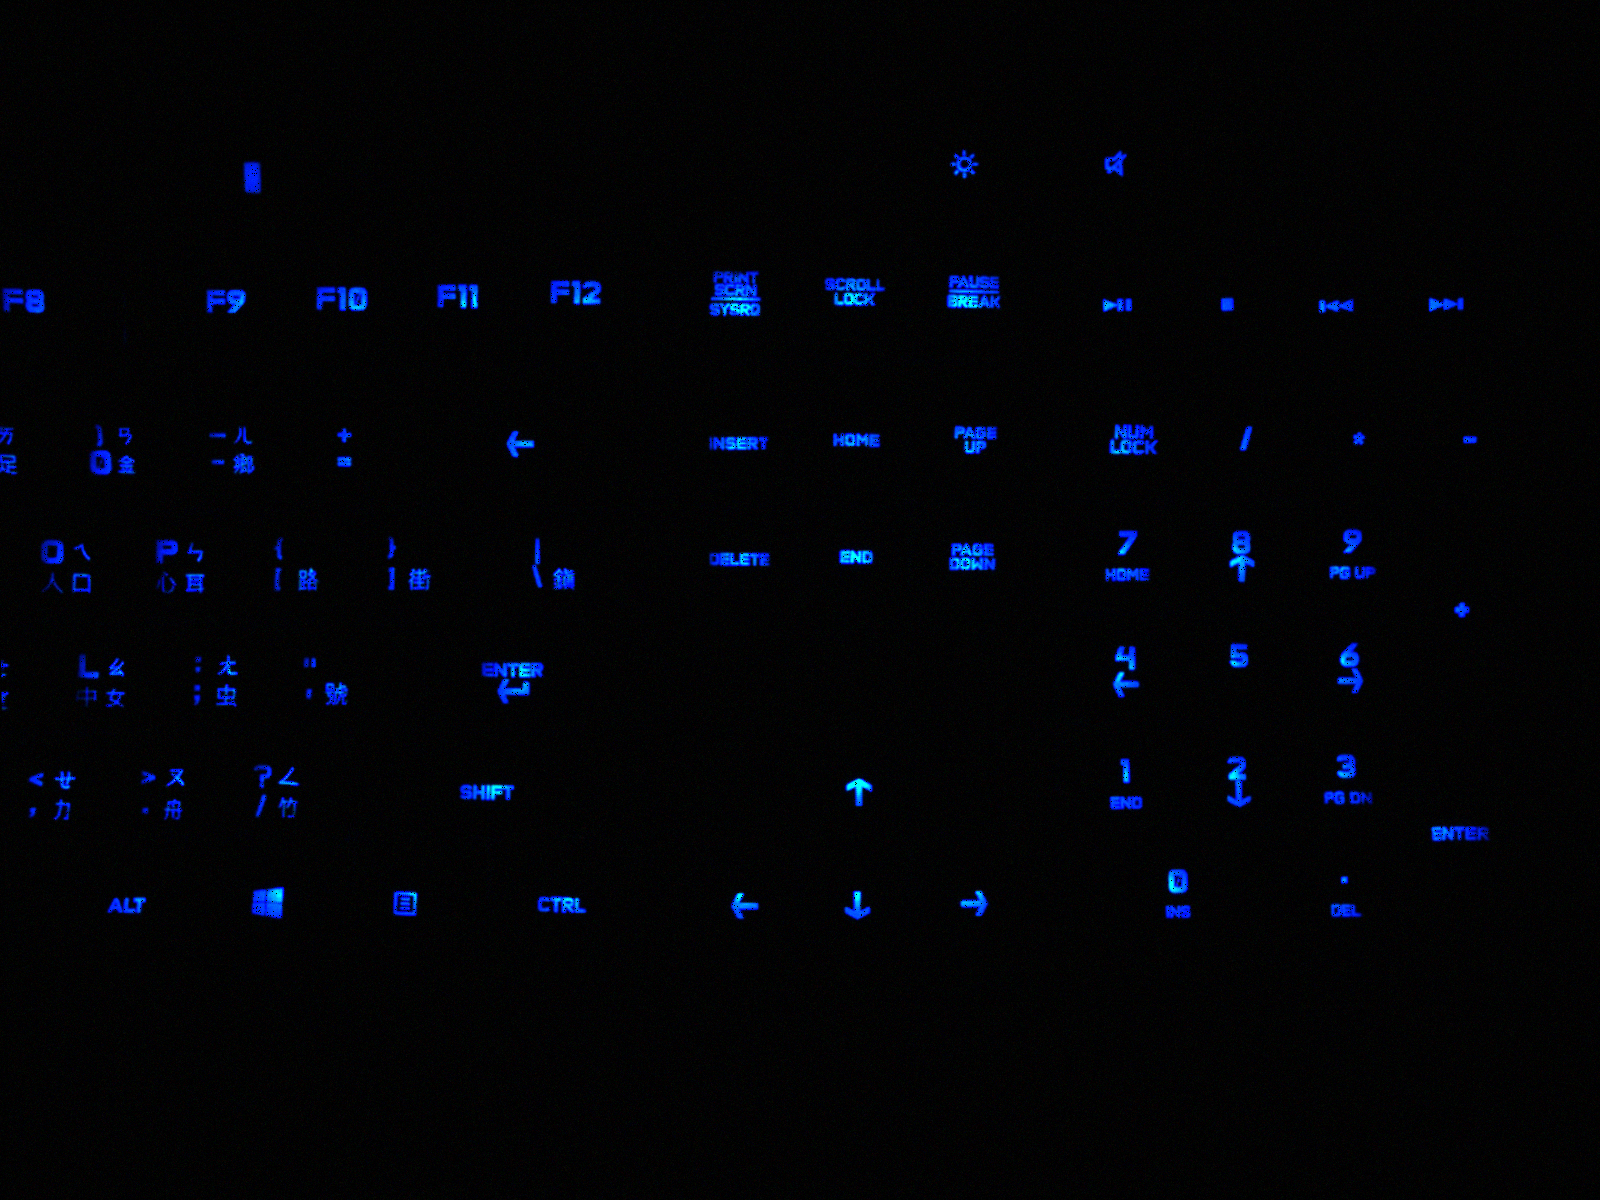
\includegraphics[width=0.5\linewidth]{simulation/normal/input_sample.png}
			}
			\caption{Input Images}
			\label{fig:RawImages}
		\end{figure}

		\subsubsection{SIFT}
		\begin{figure}[H]
			\subfigure[Reference Image Feature Points]
			{
				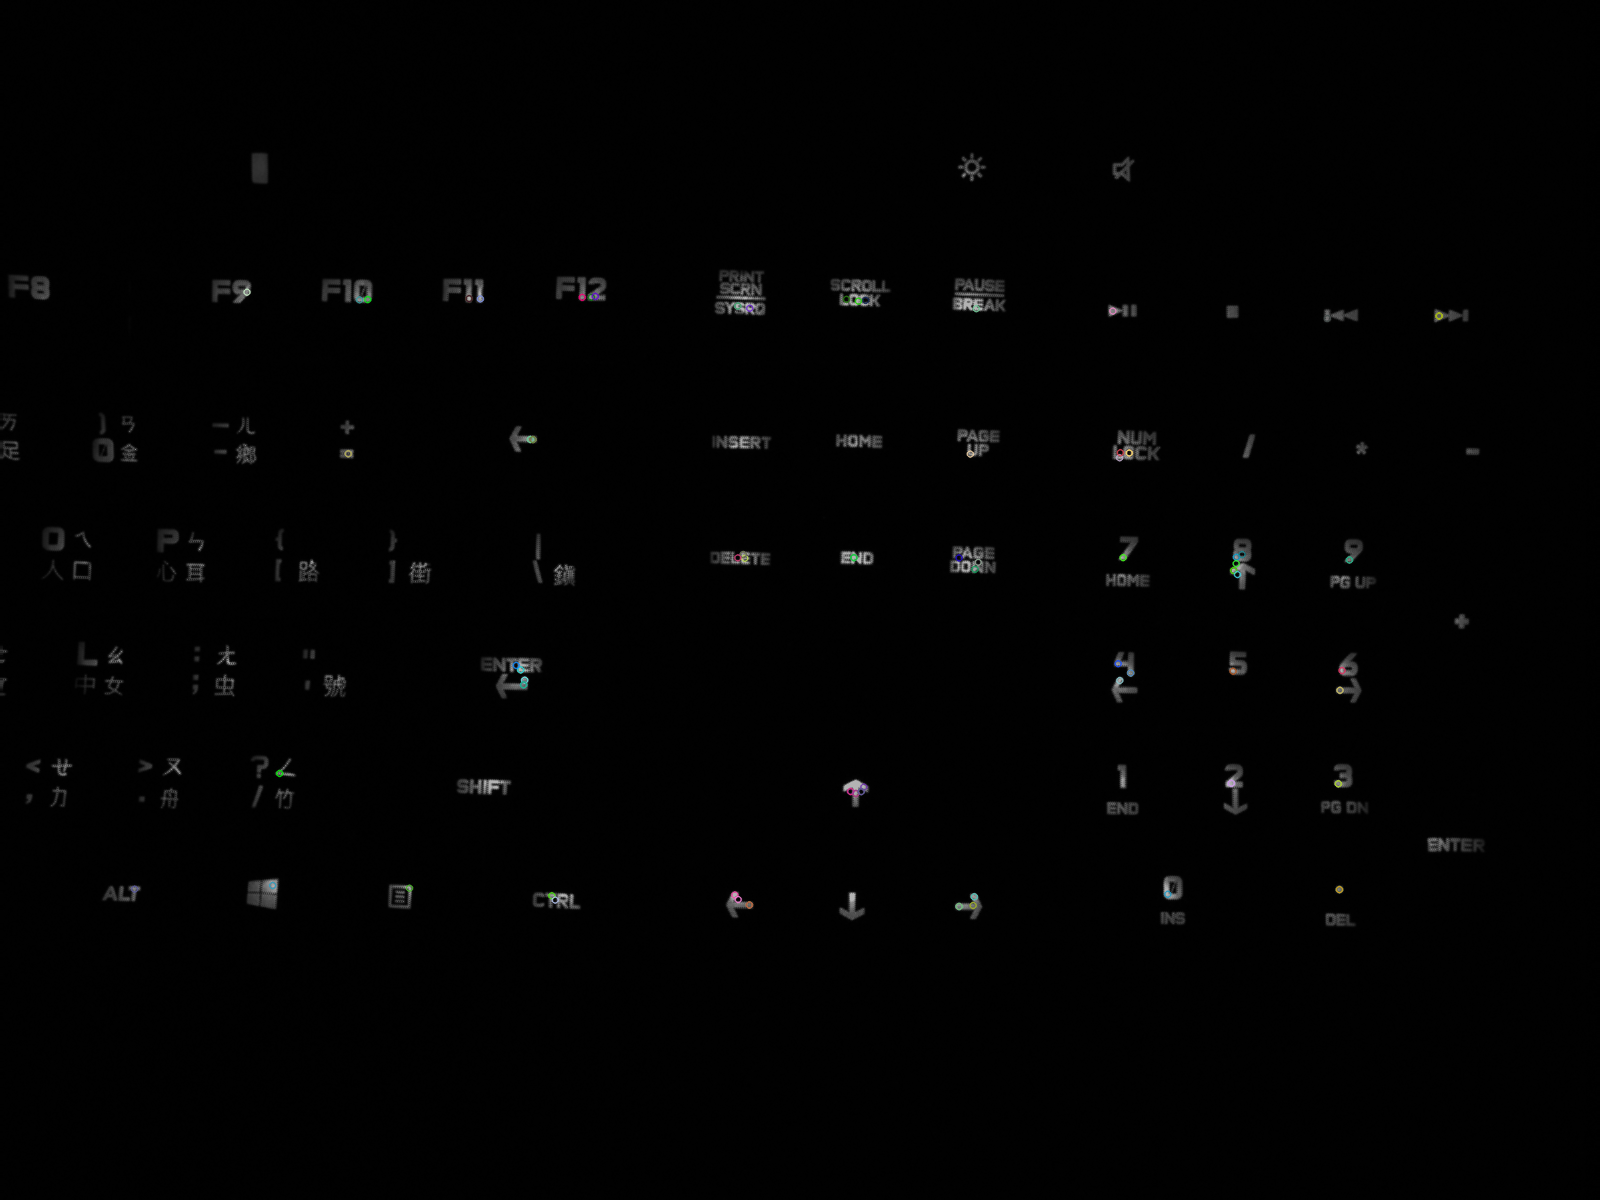
\includegraphics[width=0.5\linewidth]{simulation/normal/sift_gold_kp.png}
			}
			\subfigure[Sample Image Feature Points]
			{	
				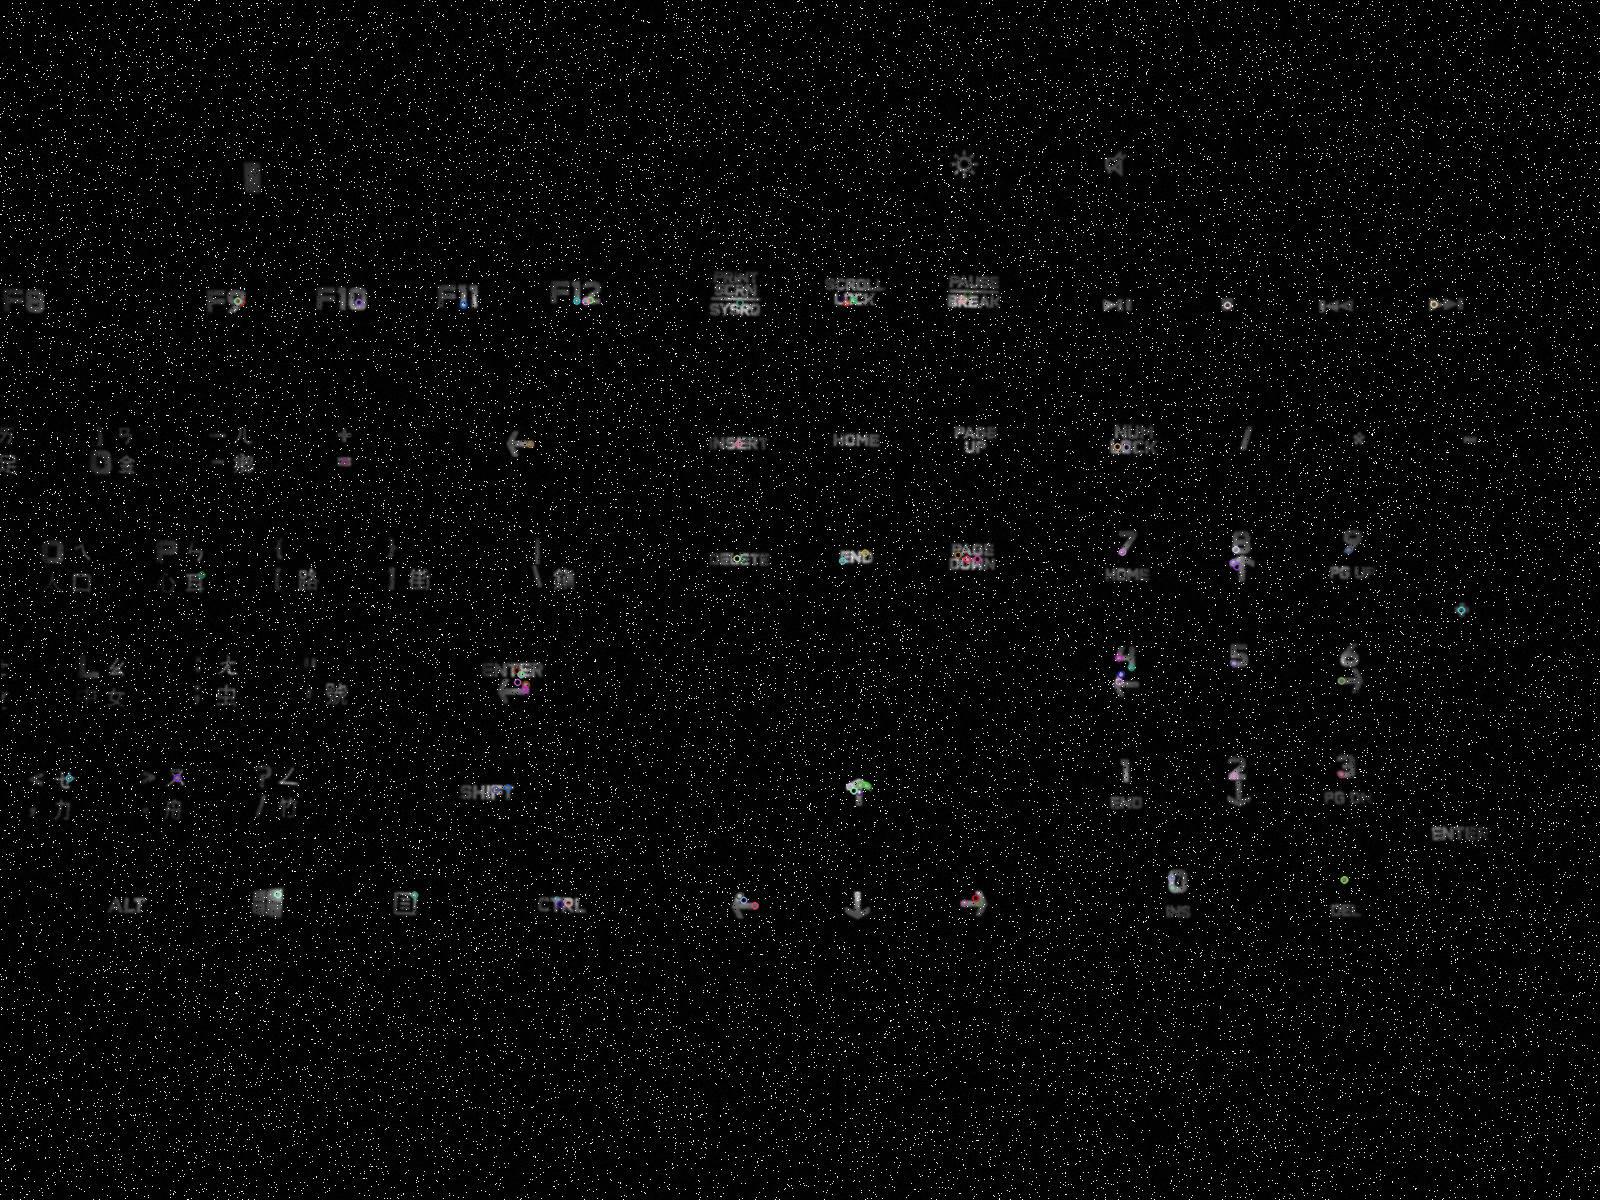
\includegraphics[width=0.5\linewidth]{simulation/normal/sift_sample_kp.png}
			}
			\caption{Reference and sample image after feature points were marked.}
			\label{fig:siftFeaturePoints}
		\end{figure}
		\begin{figure}[H]
			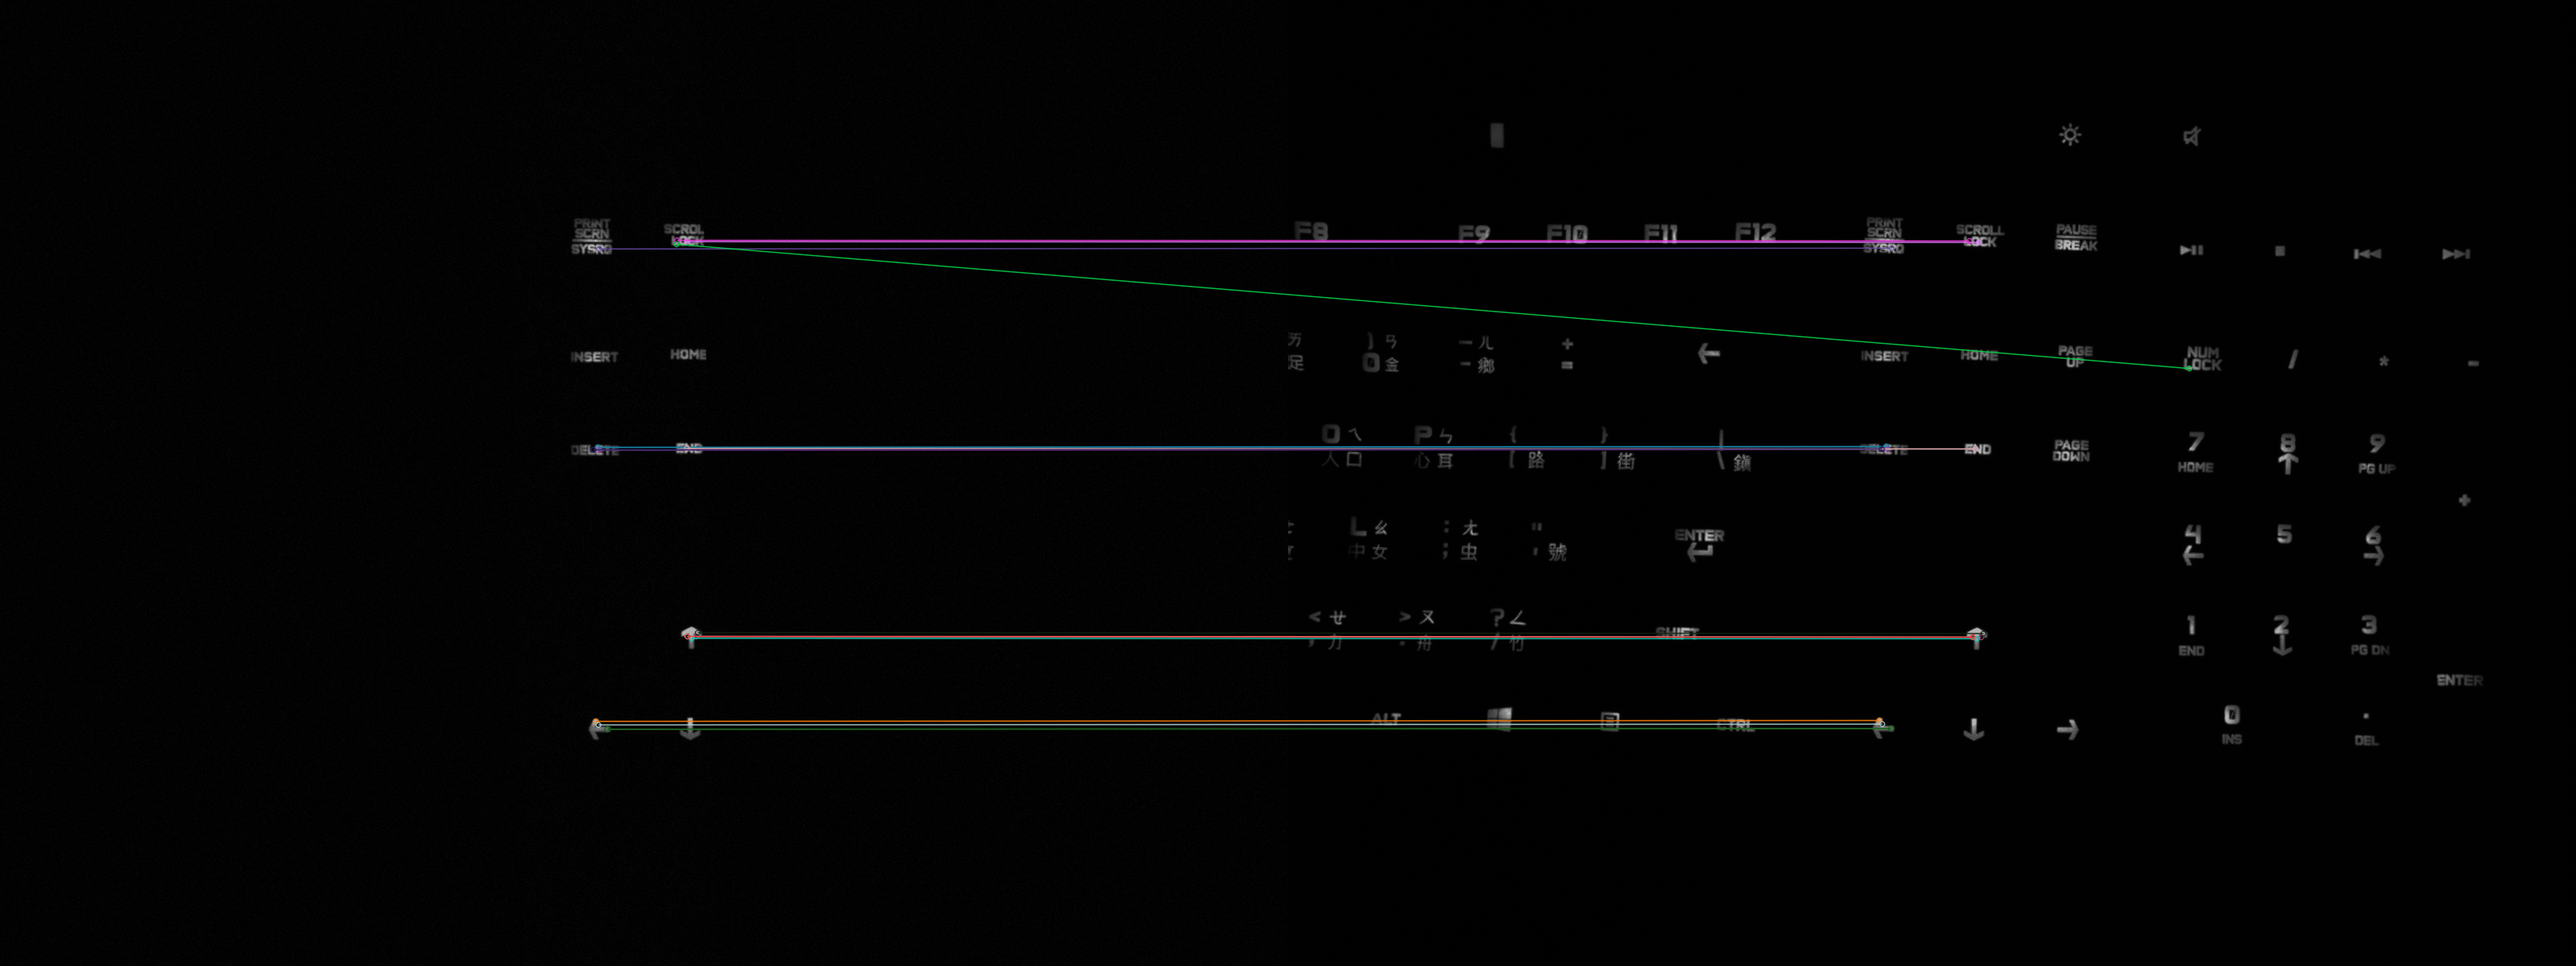
\includegraphics[width=\linewidth]{simulation/normal/sift_matches.png}
			\caption{Feature Point Matching Results}
			\label{fig:sifeMatchingResult}
		\end{figure}
		\begin{figure}[H]
			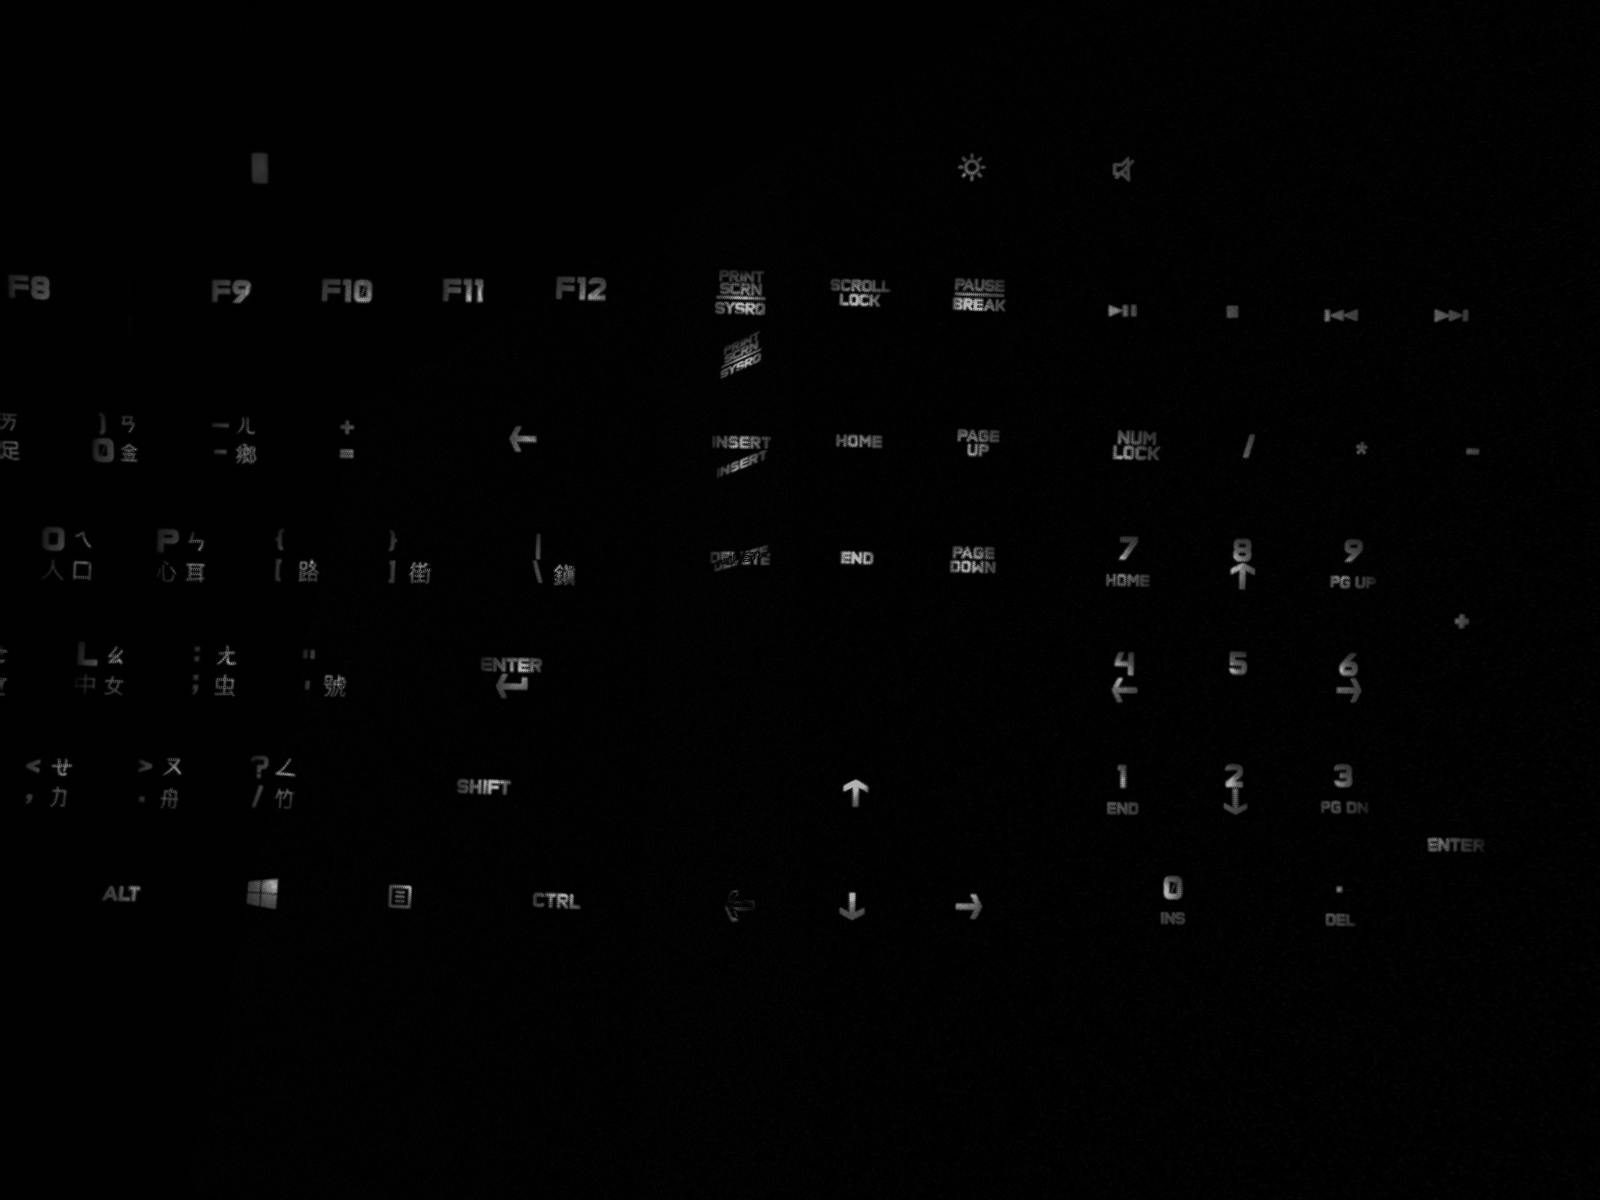
\includegraphics[width=\linewidth]{simulation/normal/sift_absdiff.png}
			\caption{Absolute Difference Results}
			\label{fig:siftAbsDifference}
		\end{figure}


		\subsubsection{SURF}
		\begin{figure}[H]
			\subfigure[Reference Image Feature Points]
			{
				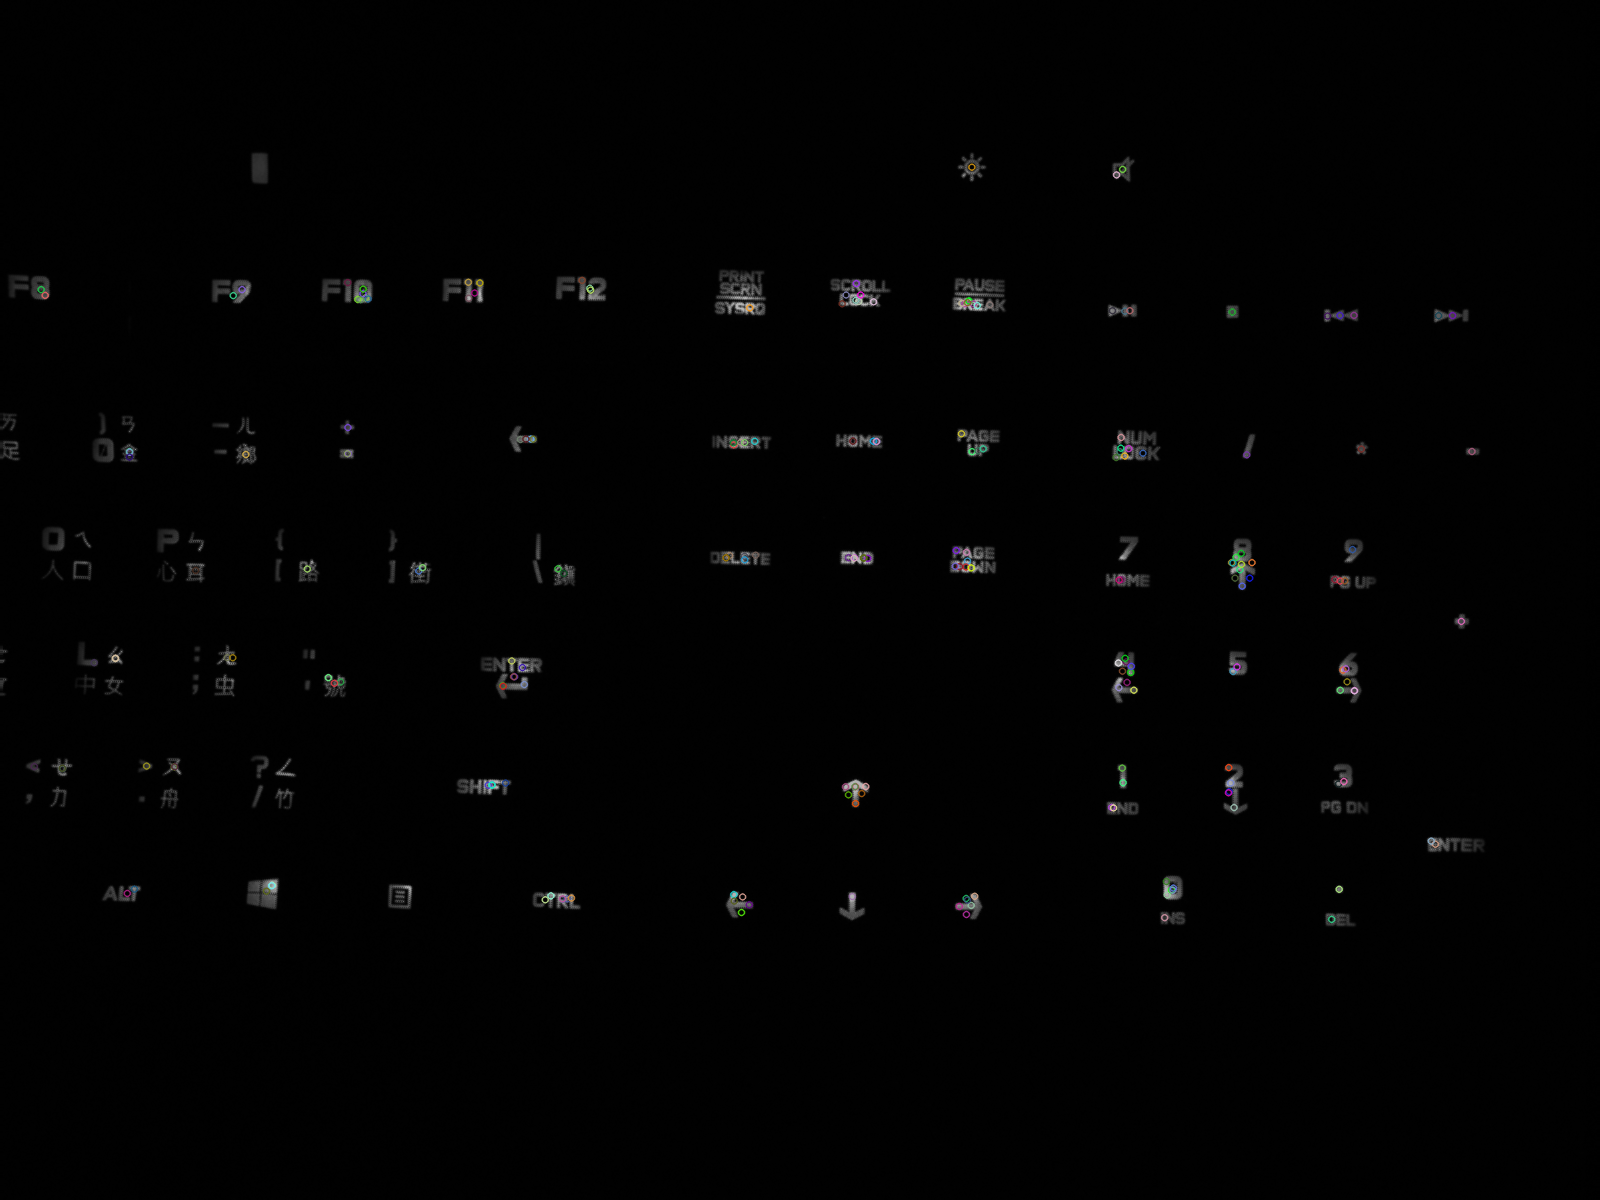
\includegraphics[width=0.5\linewidth]{simulation/normal/surf_gold_kp.png}
			}
			\subfigure[Sample Image Feature Points]
			{	
				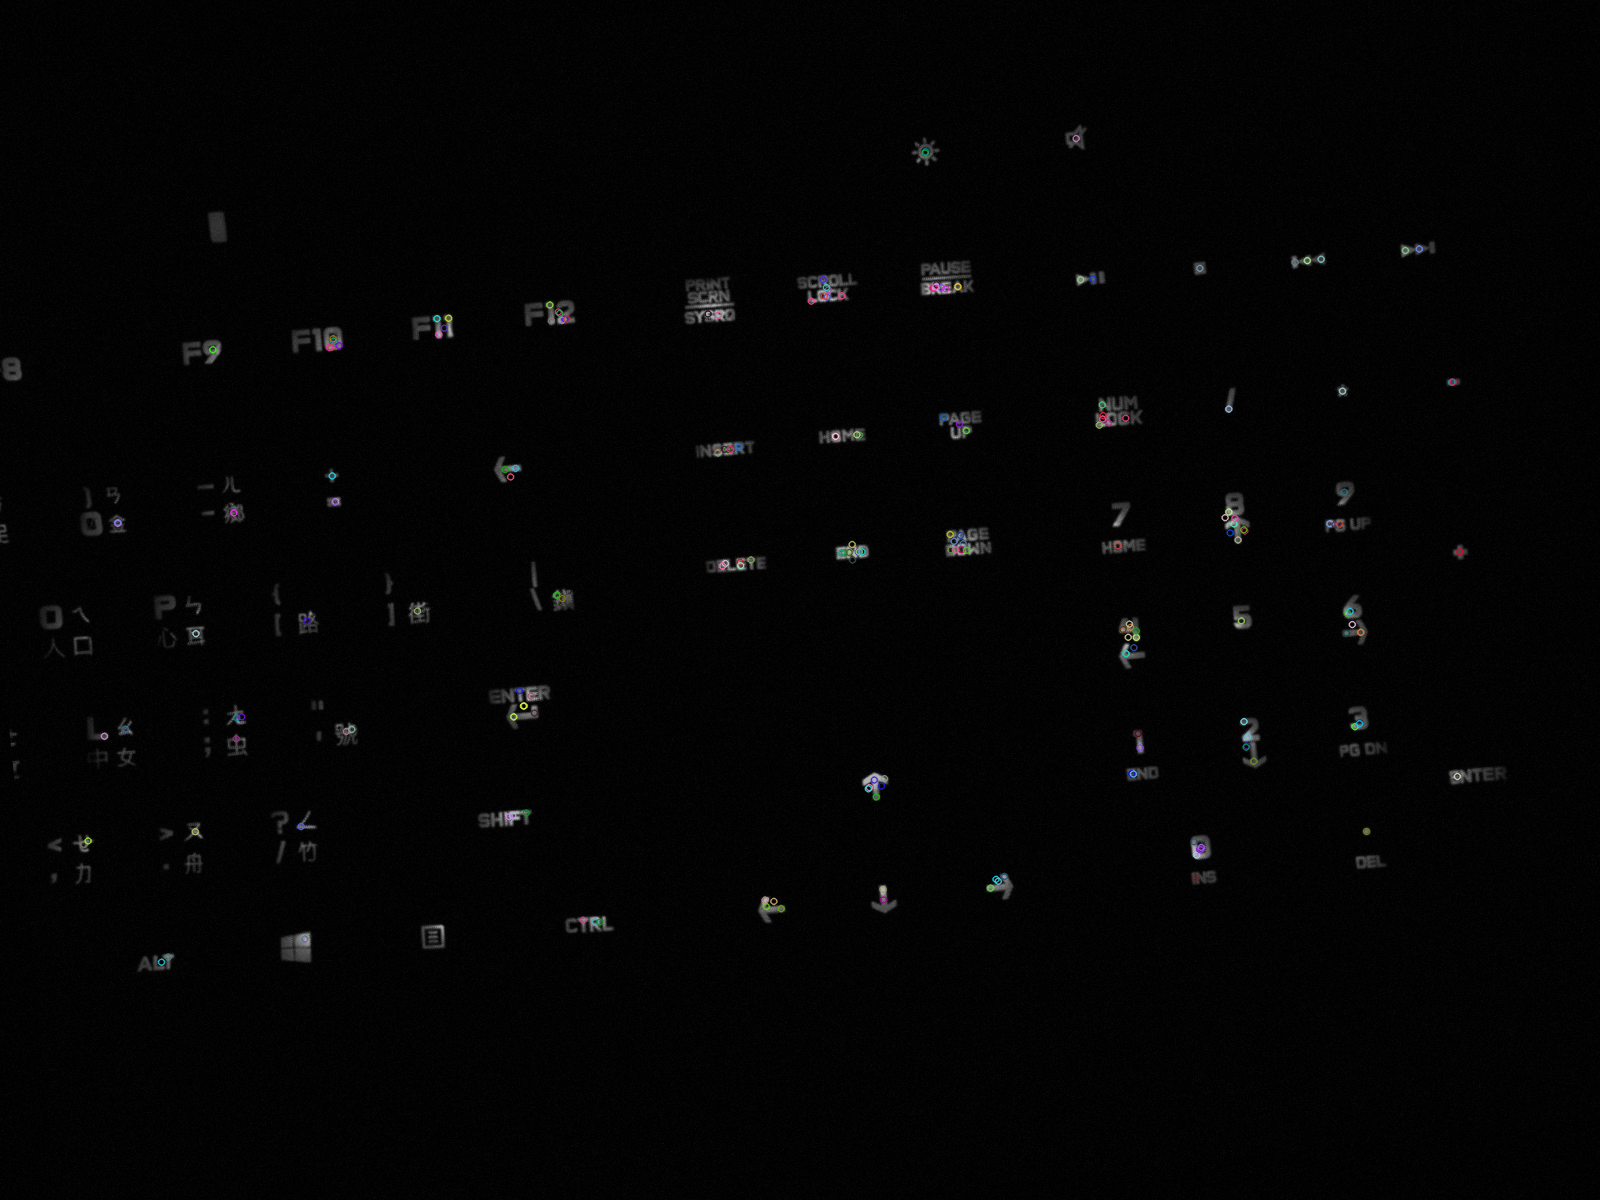
\includegraphics[width=0.5\linewidth]{simulation/normal/surf_sample_kp.png}
			}
			\caption{Reference and sample image after feature points were marked.}
			\label{fig:siftFeaturePoints}
		\end{figure}
		\begin{figure}[H]
			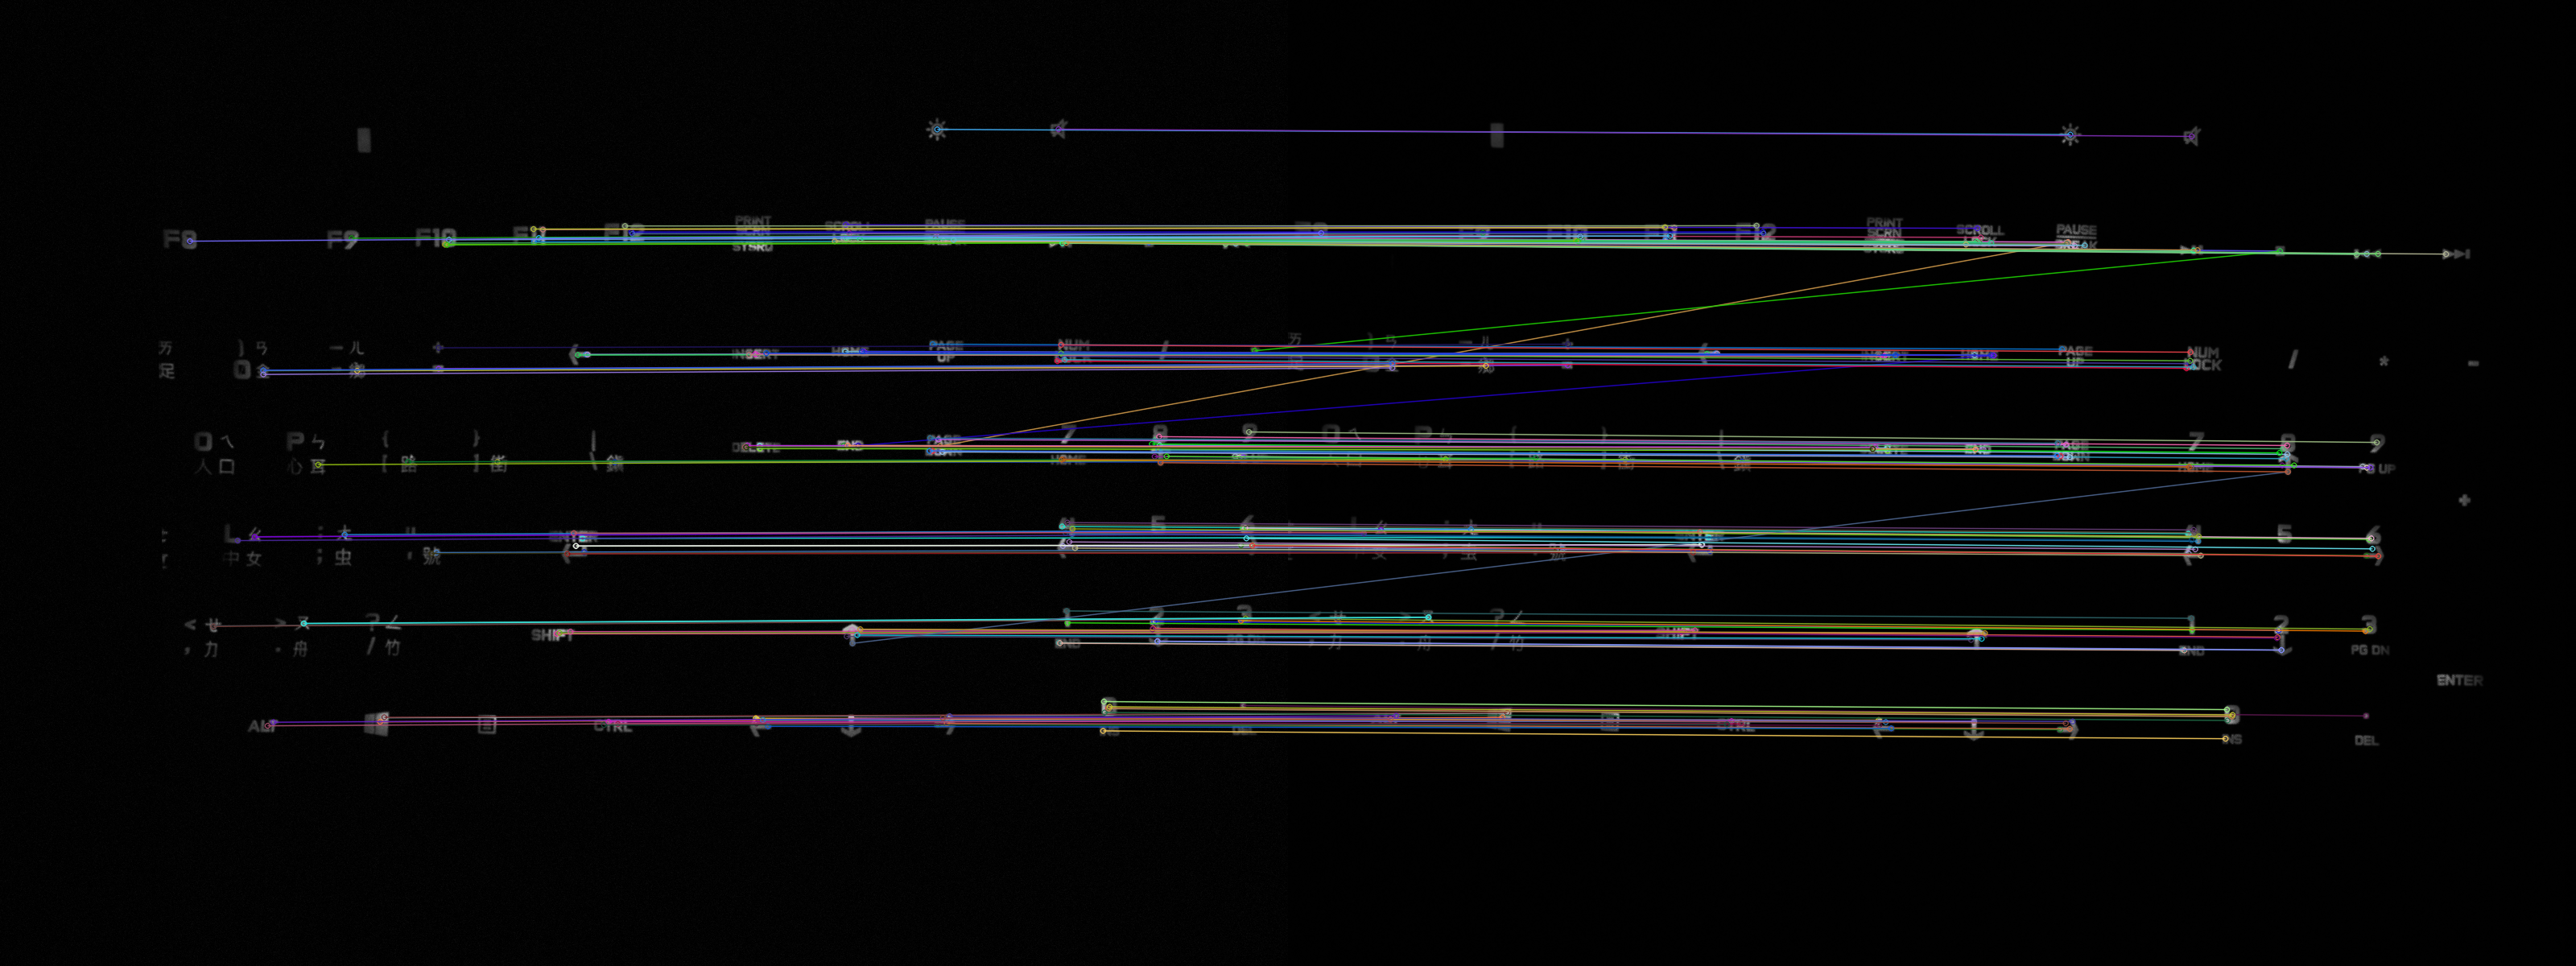
\includegraphics[width=\linewidth]{simulation/normal/surf_matches.png}
			\caption{Feature Point Matching Results}
			\label{fig:sifeMatchingResult}
		\end{figure}
		\begin{figure}[H]
			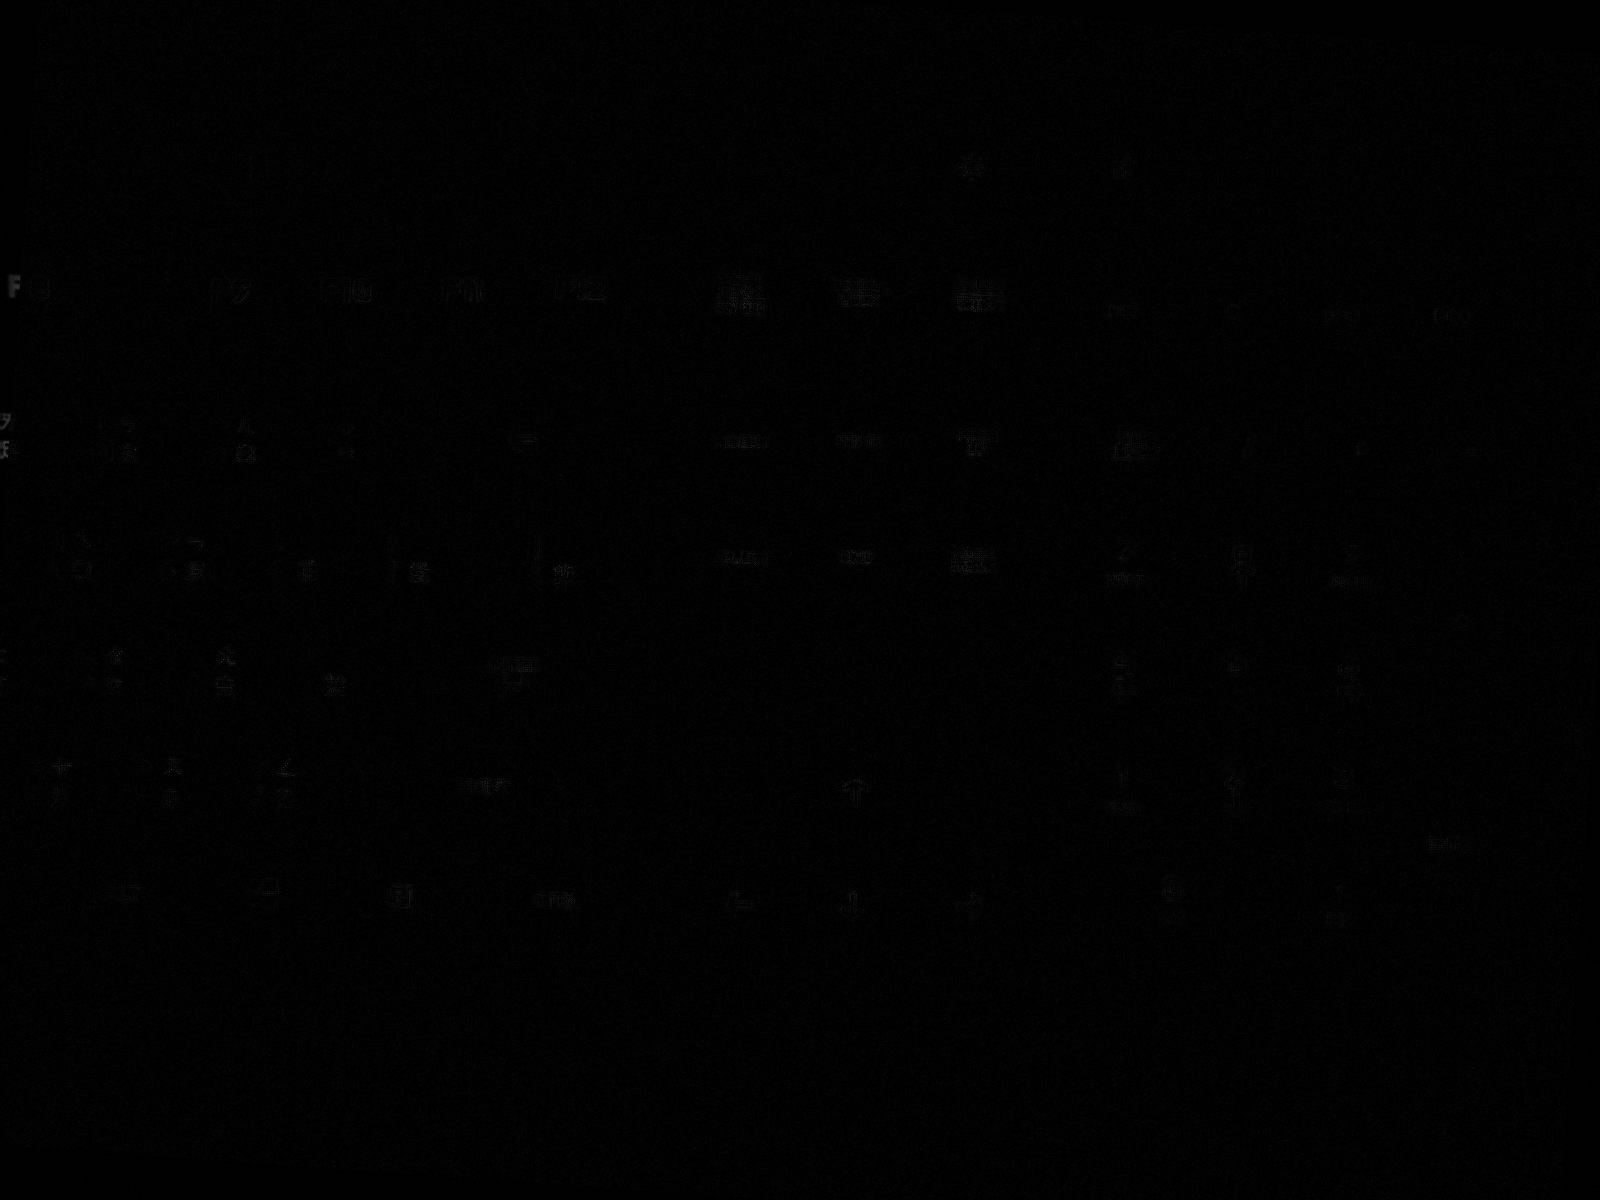
\includegraphics[width=\linewidth]{simulation/normal/surf_absdiff.png}
			\caption{Absolute Difference Results}
			\label{fig:siftAbsDifference}
		\end{figure}


		\subsubsection{ORB}
		\begin{figure}[H]
			\subfigure[Reference Image Feature Points]
			{
				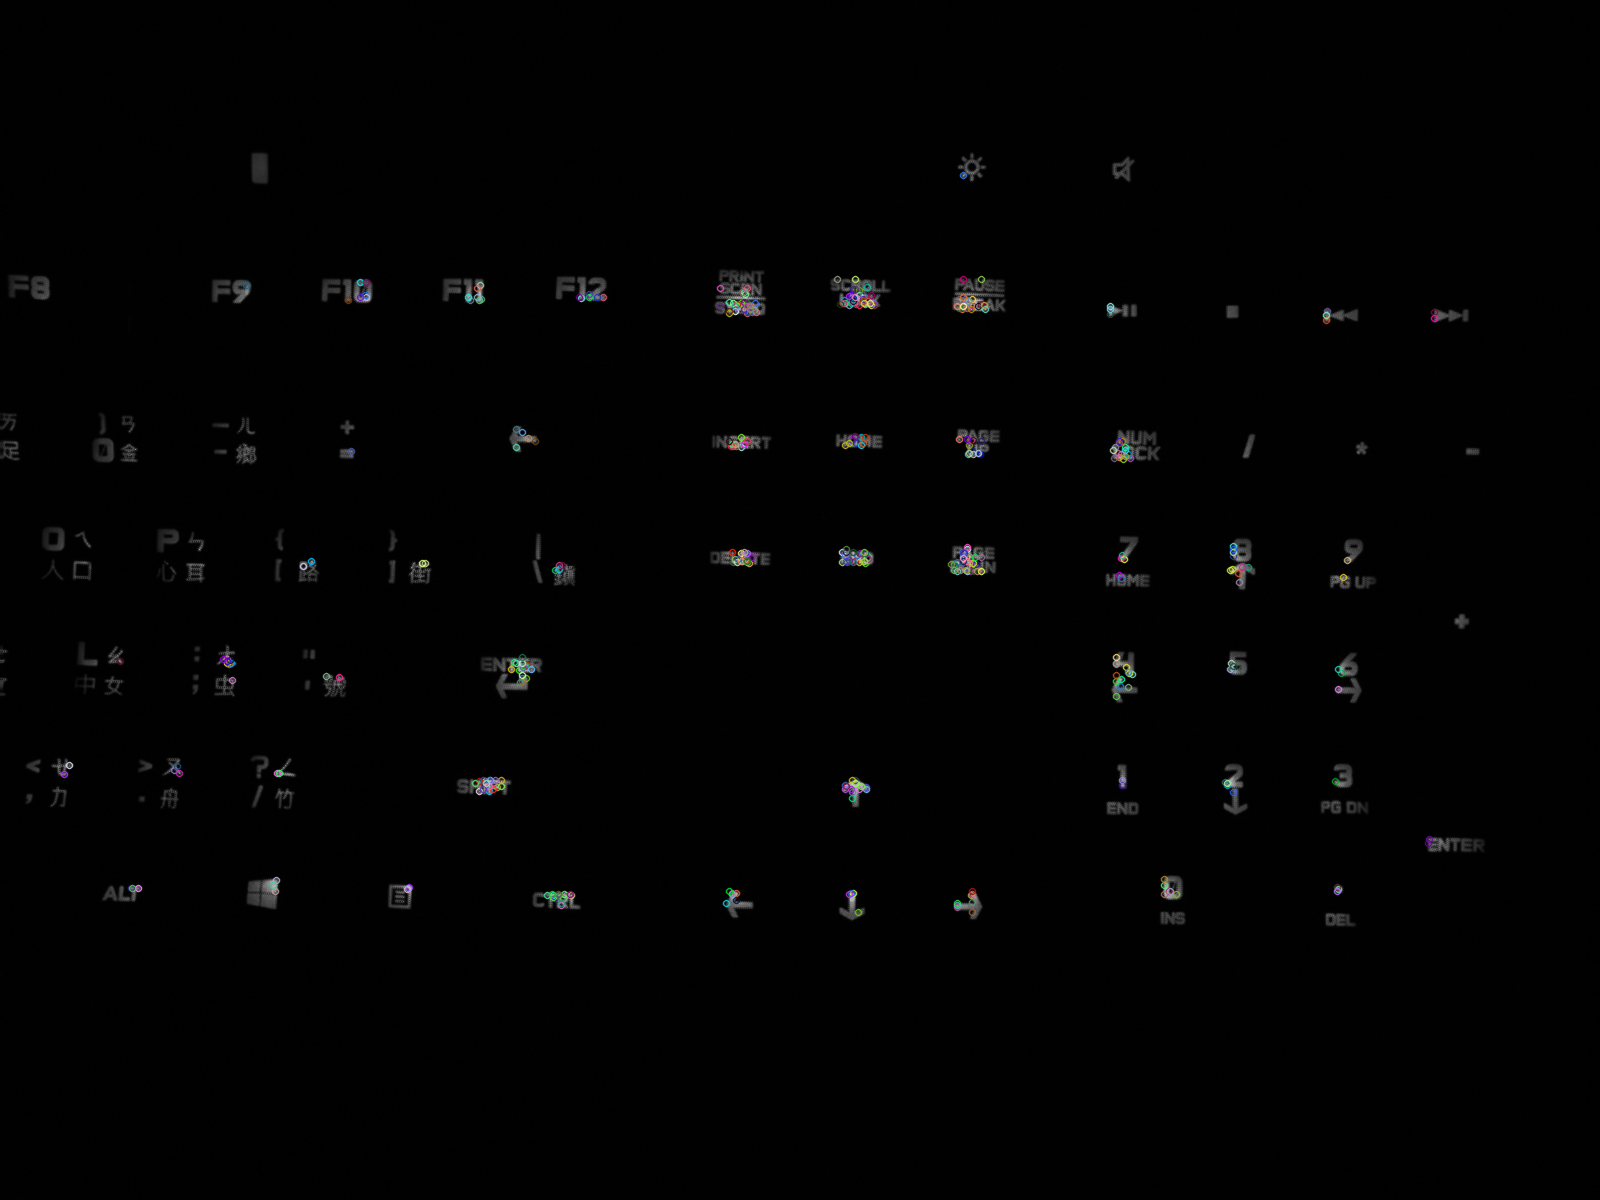
\includegraphics[width=0.5\linewidth]{simulation/normal/orb_gold_kp.png}
			}
			\subfigure[Sample Image Feature Points]
			{	
				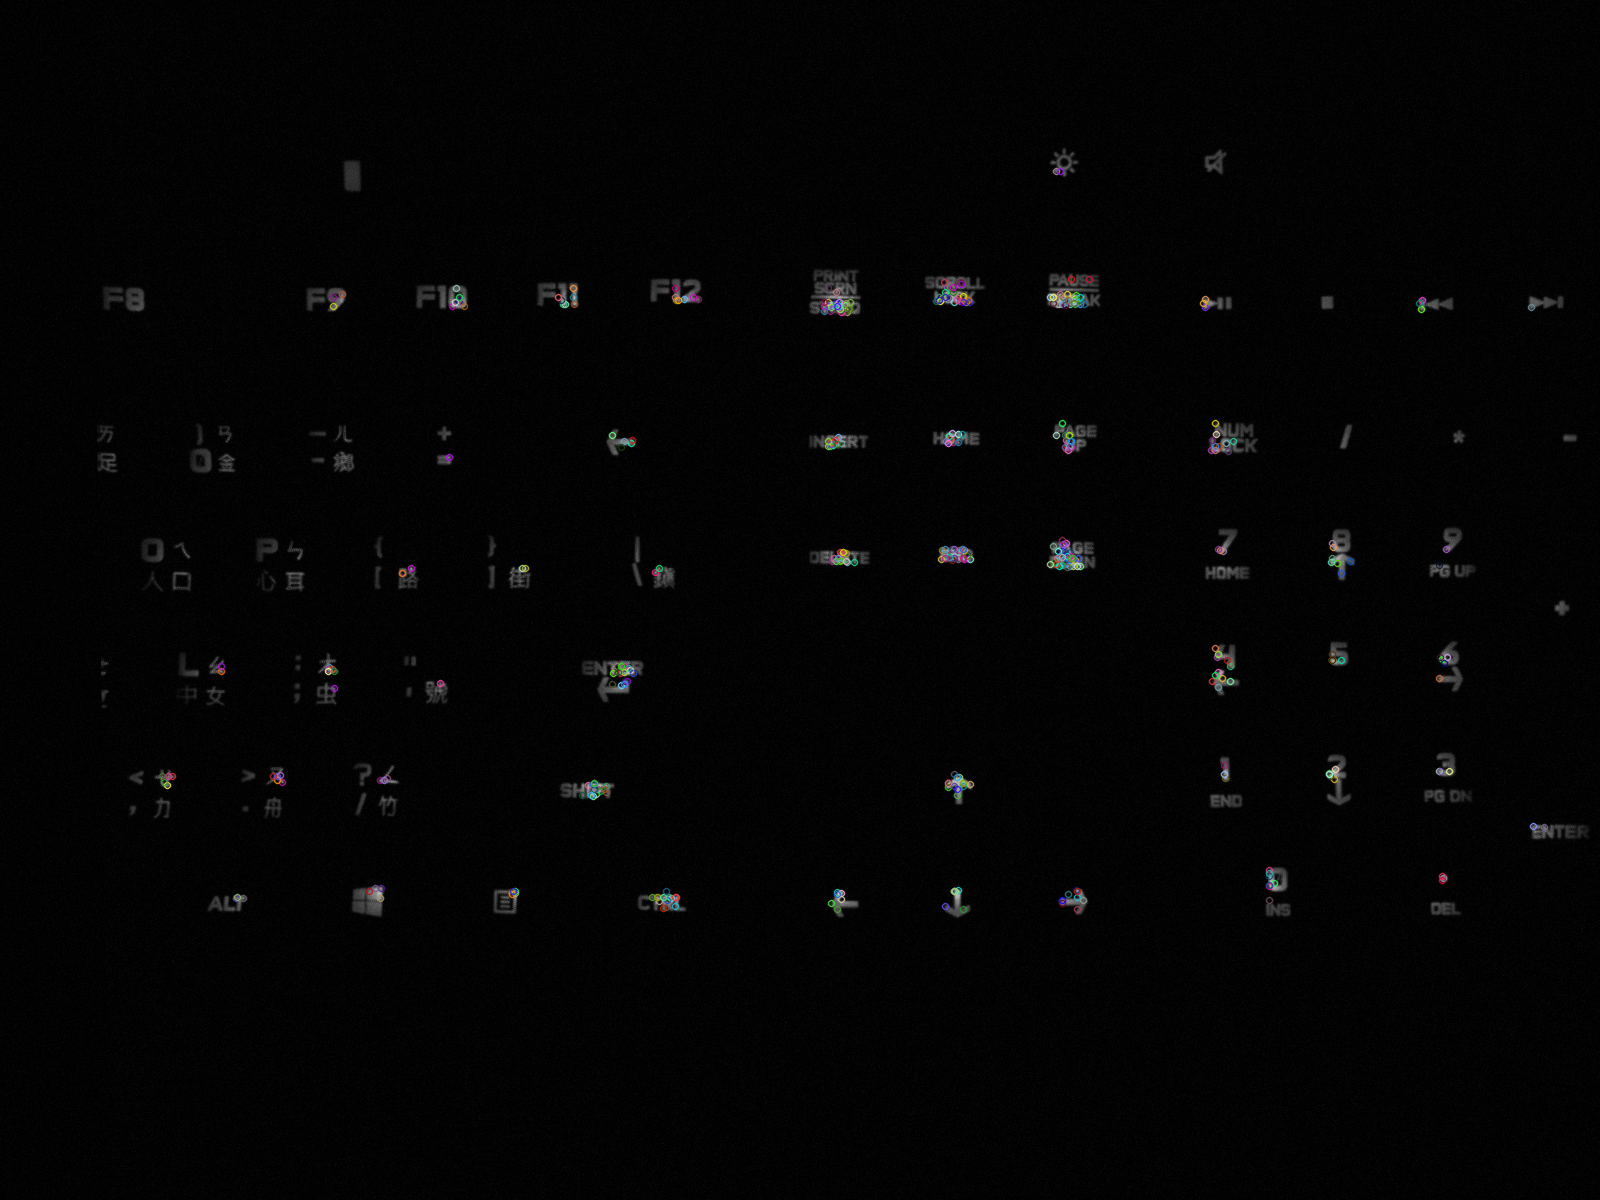
\includegraphics[width=0.5\linewidth]{simulation/normal/orb_sample_kp.png}
			}
			\caption{Reference and sample image after feature points were marked.}
			\label{fig:siftFeaturePoints}
		\end{figure}
		\begin{figure}[H]
			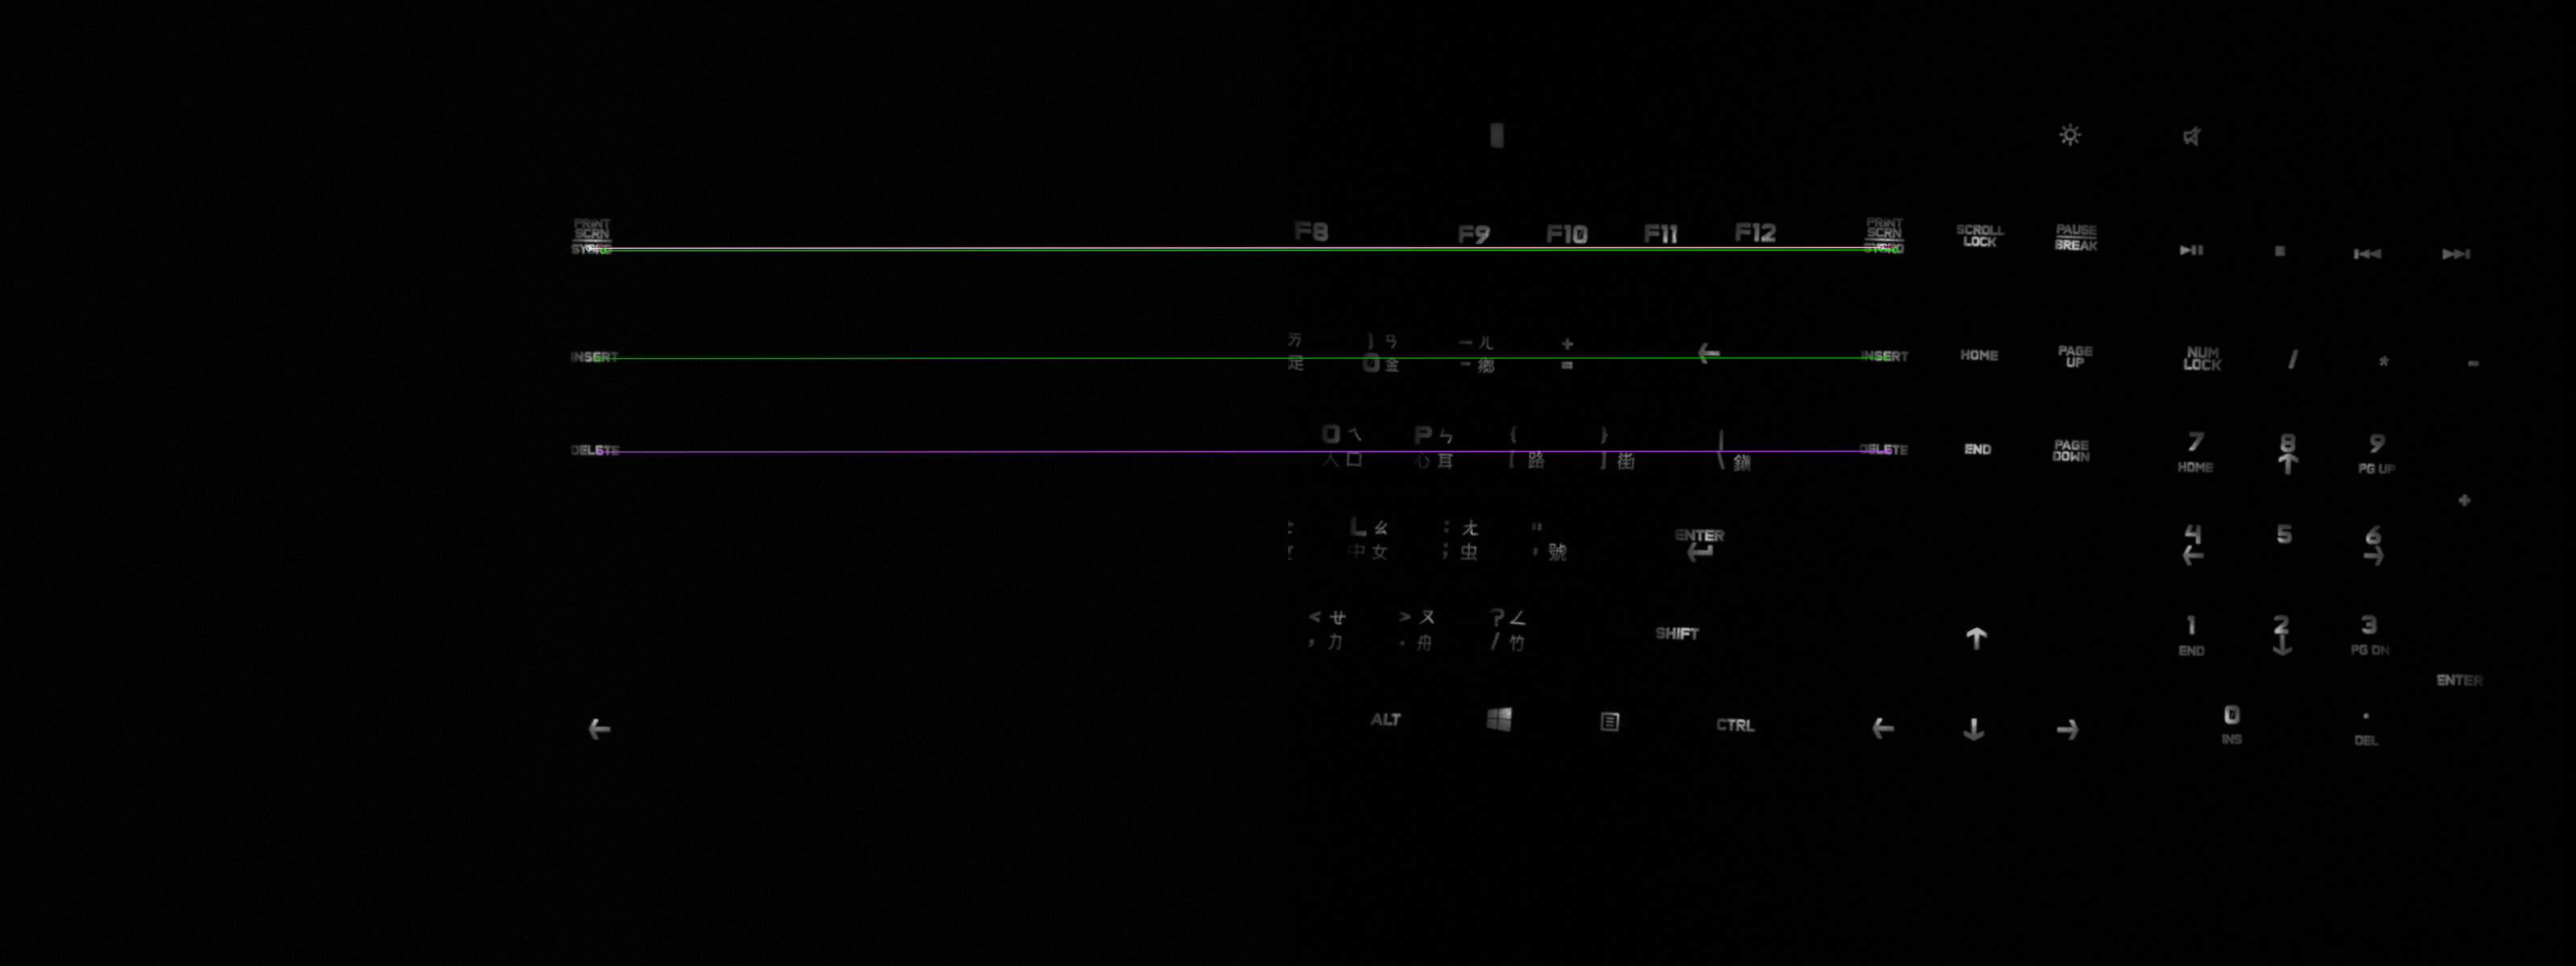
\includegraphics[width=\linewidth]{simulation/normal/orb_matches.png}
			\caption{Feature Point Matching Results}
			\label{fig:sifeMatchingResult}
		\end{figure}
		\begin{figure}[H]
			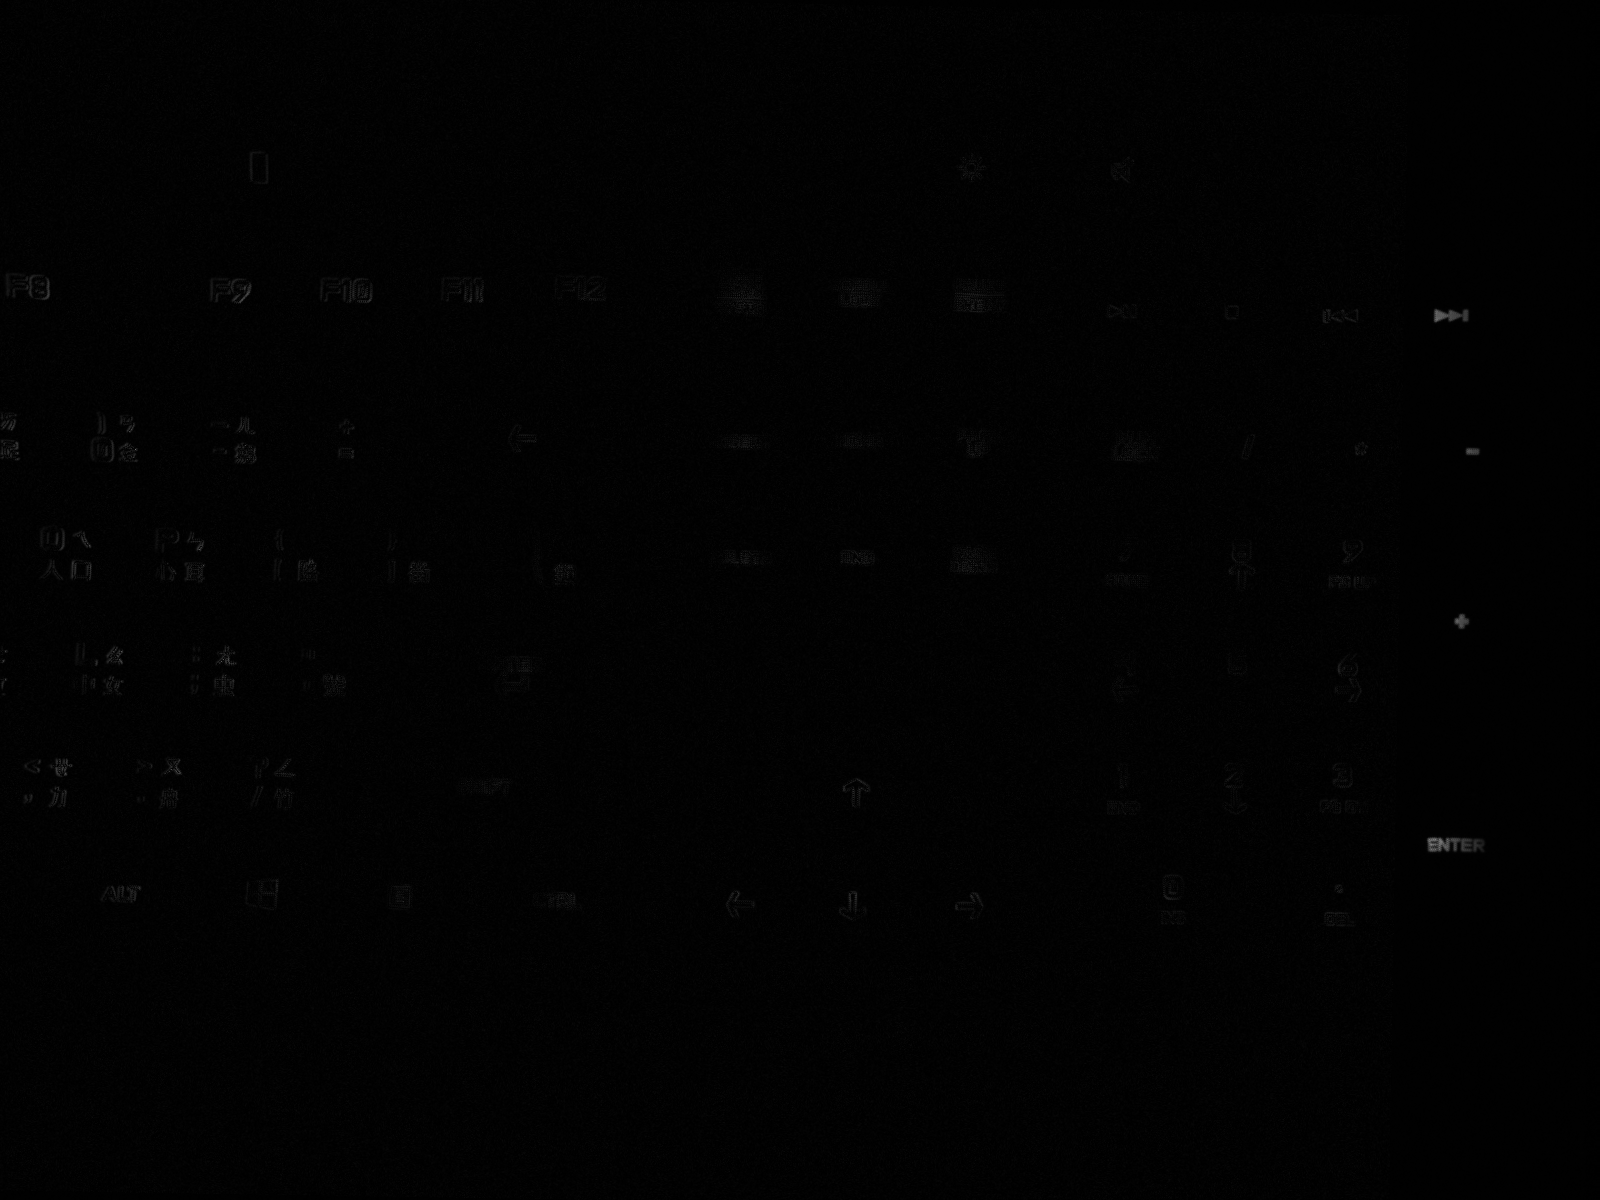
\includegraphics[width=\linewidth]{simulation/normal/orb_absdiff.png}
			\caption{Absolute Difference Results}
			\label{fig:siftAbsDifference}
		\end{figure}

		\subsubsection{AKAZE}
		\begin{figure}[H]
			\subfigure[Reference Image Feature Points]
			{
				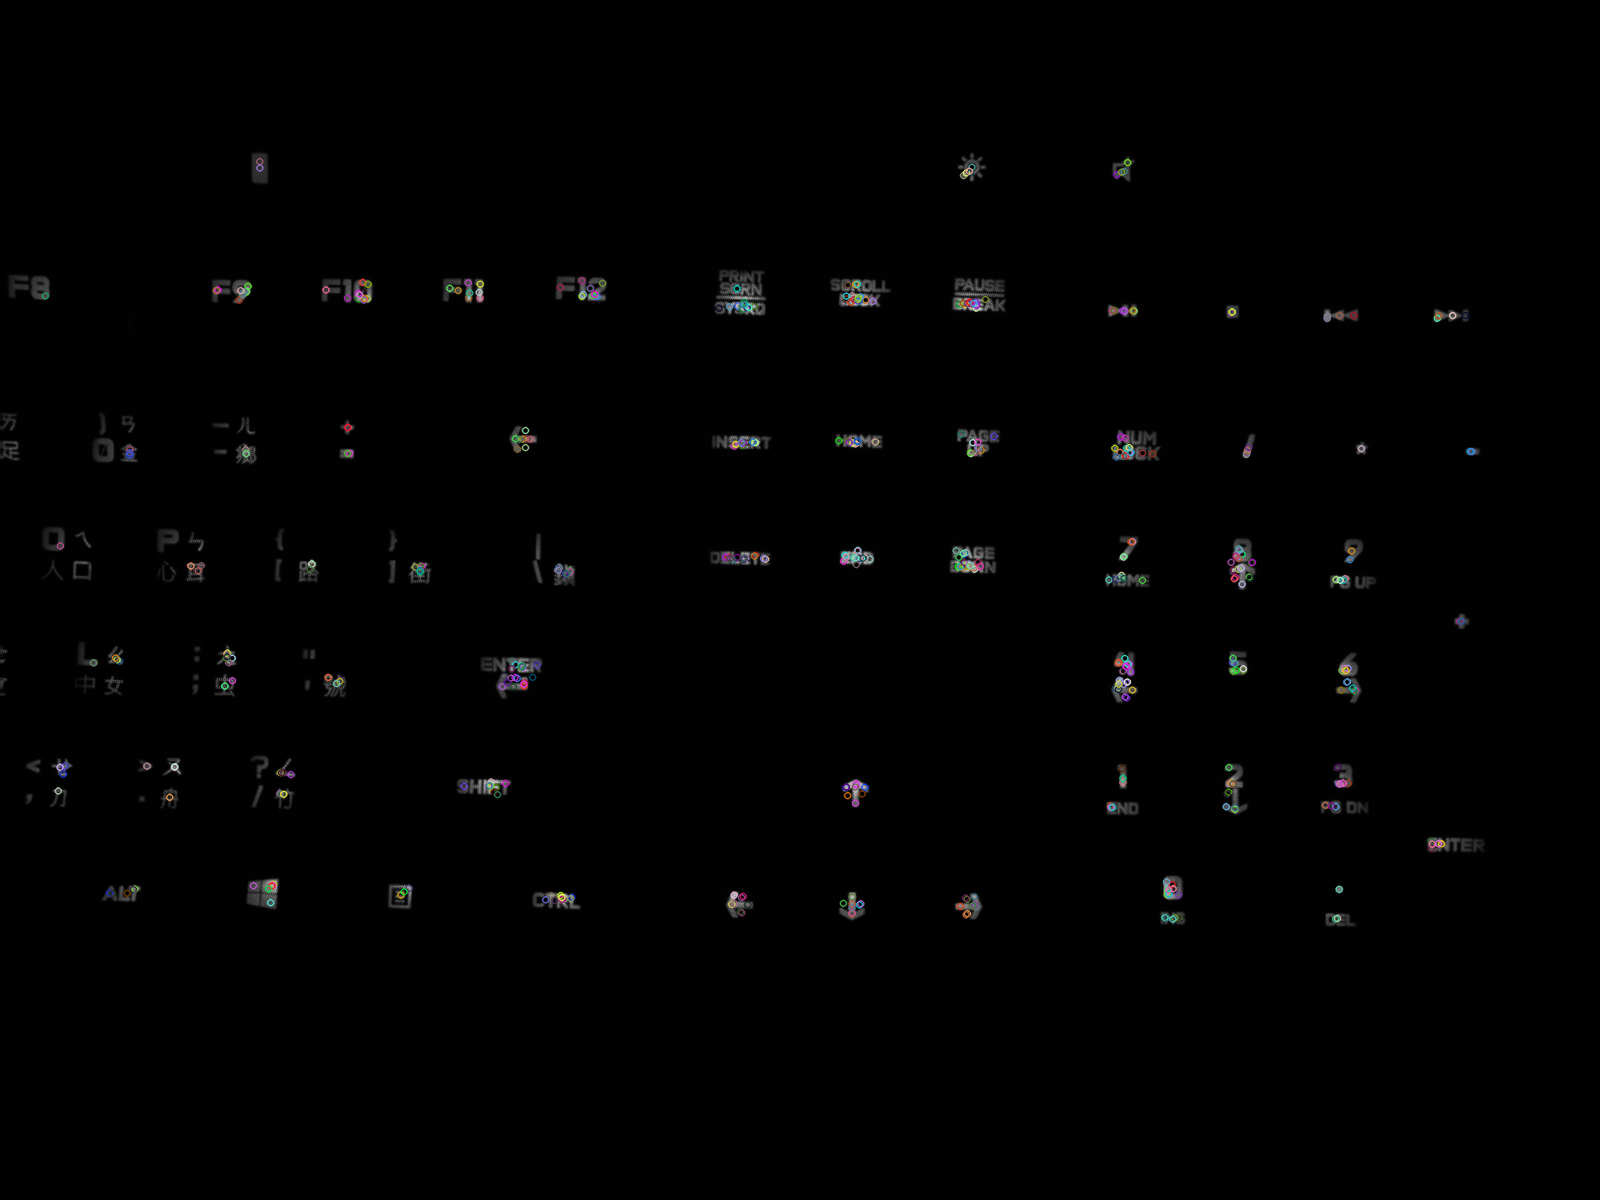
\includegraphics[width=0.5\linewidth]{simulation/normal/akaze_gold_kp.png}
			}
			\subfigure[Sample Image Feature Points]
			{	
				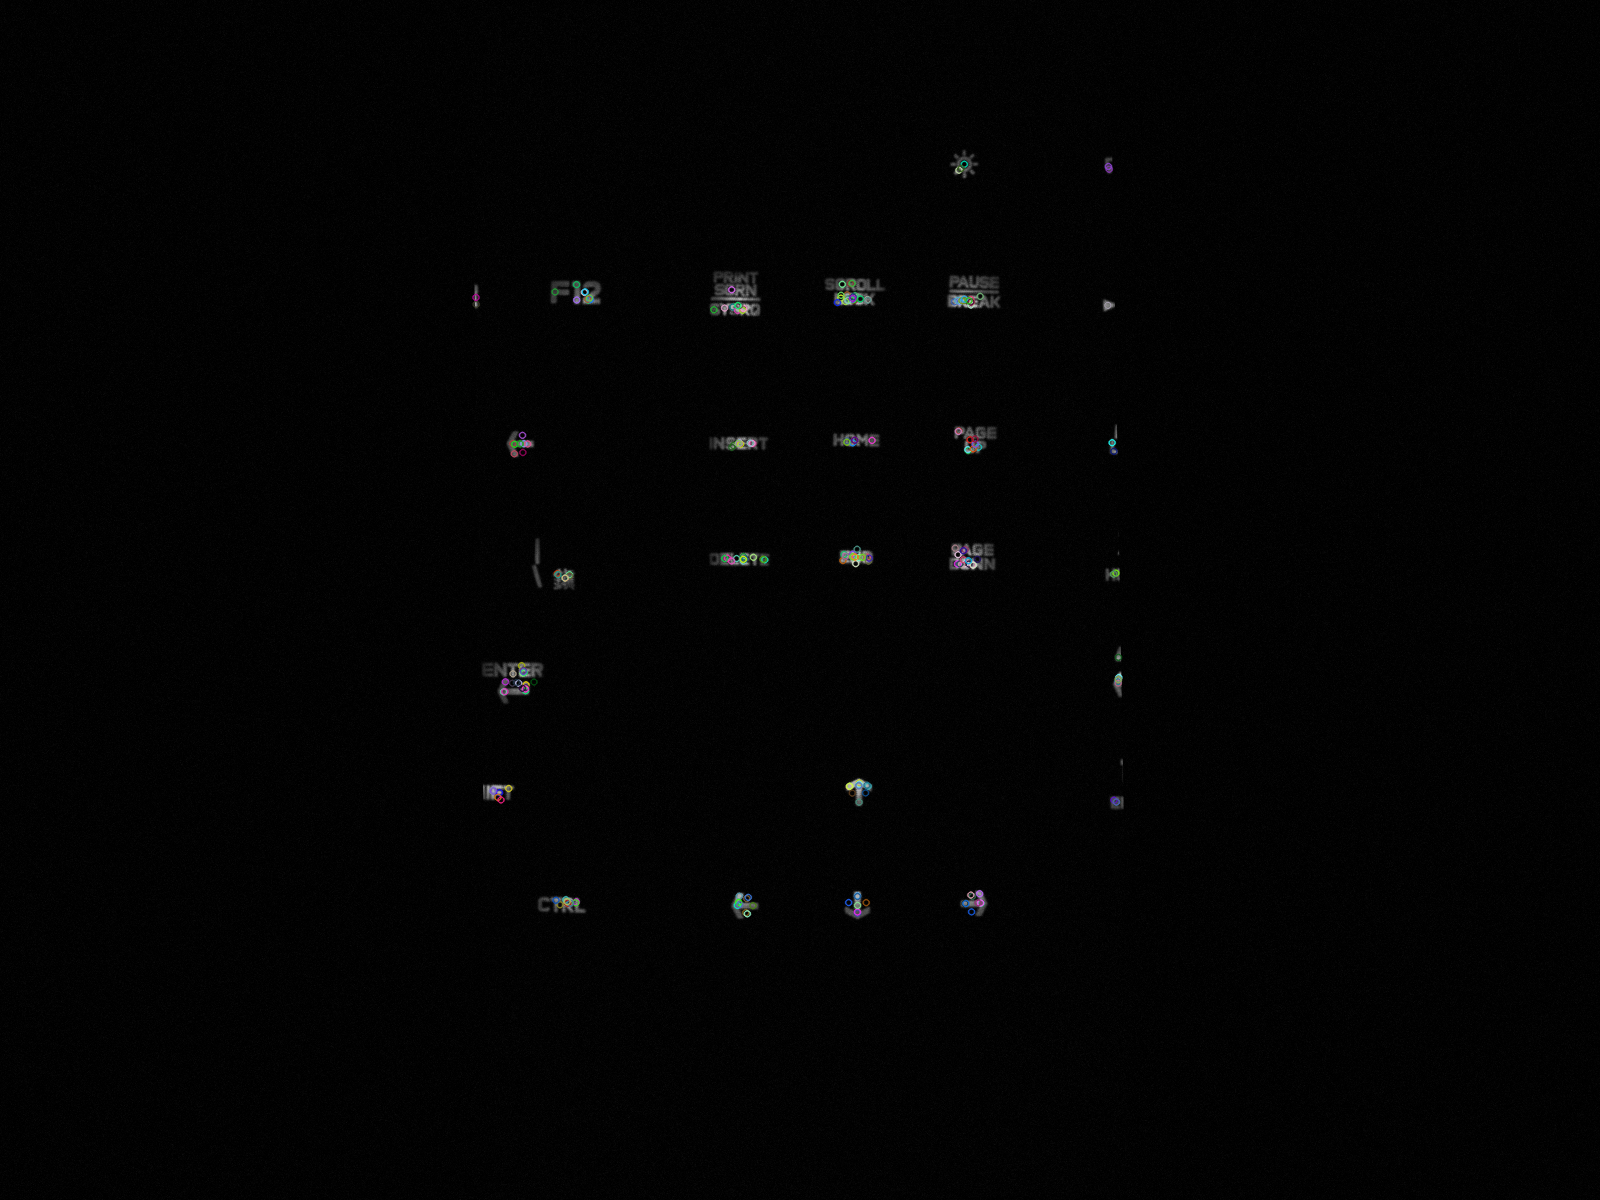
\includegraphics[width=0.5\linewidth]{simulation/normal/akaze_sample_kp.png}
			}
			\caption{Reference and sample image after feature points were marked.}
			\label{fig:siftFeaturePoints}
		\end{figure}
		\begin{figure}[H]
			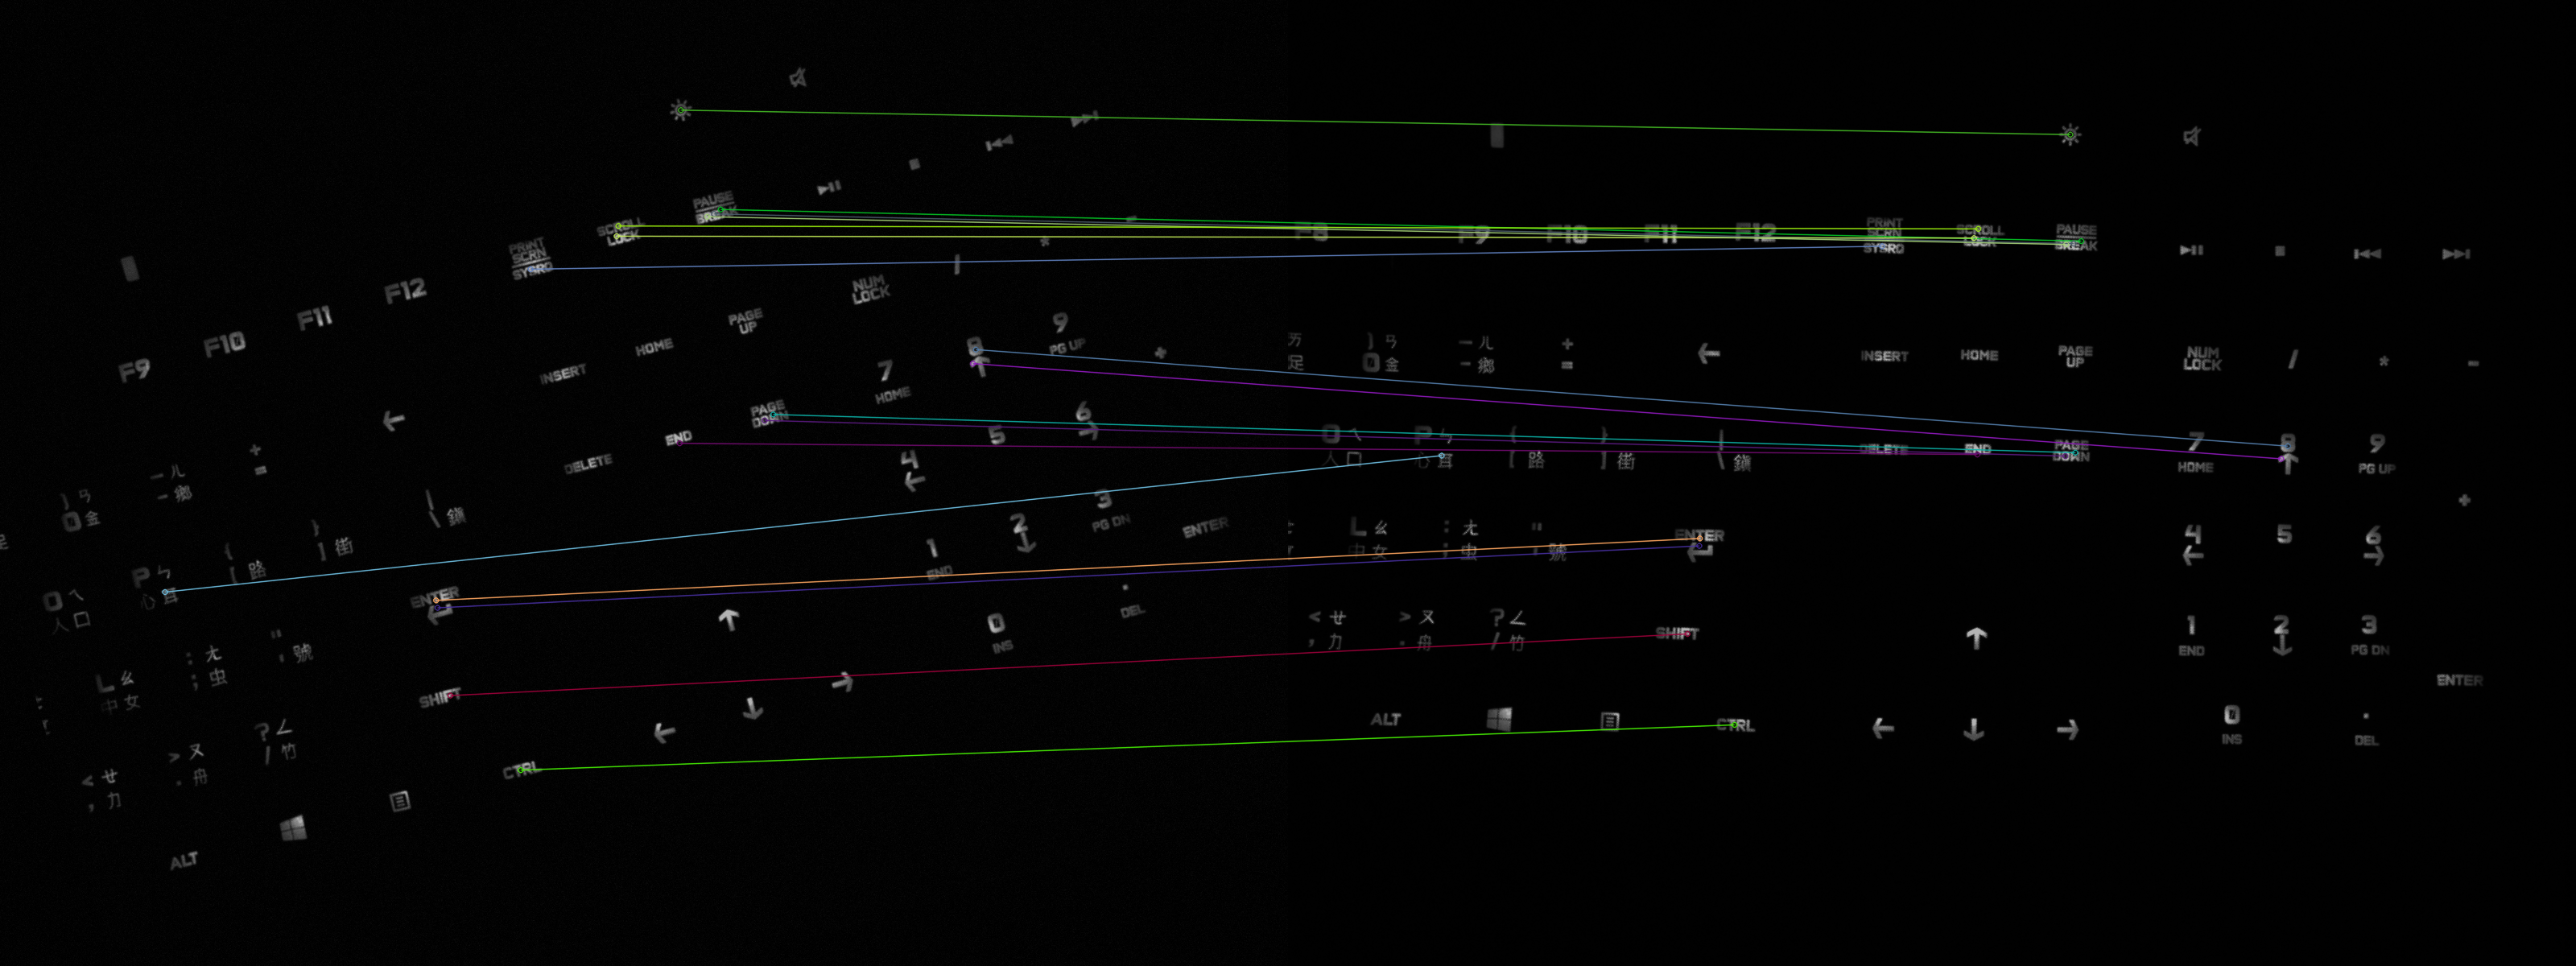
\includegraphics[width=\linewidth]{simulation/normal/akaze_matches.png}
			\caption{Feature Point Matching Results}
			\label{fig:sifeMatchingResult}
		\end{figure}
		\begin{figure}[H]
			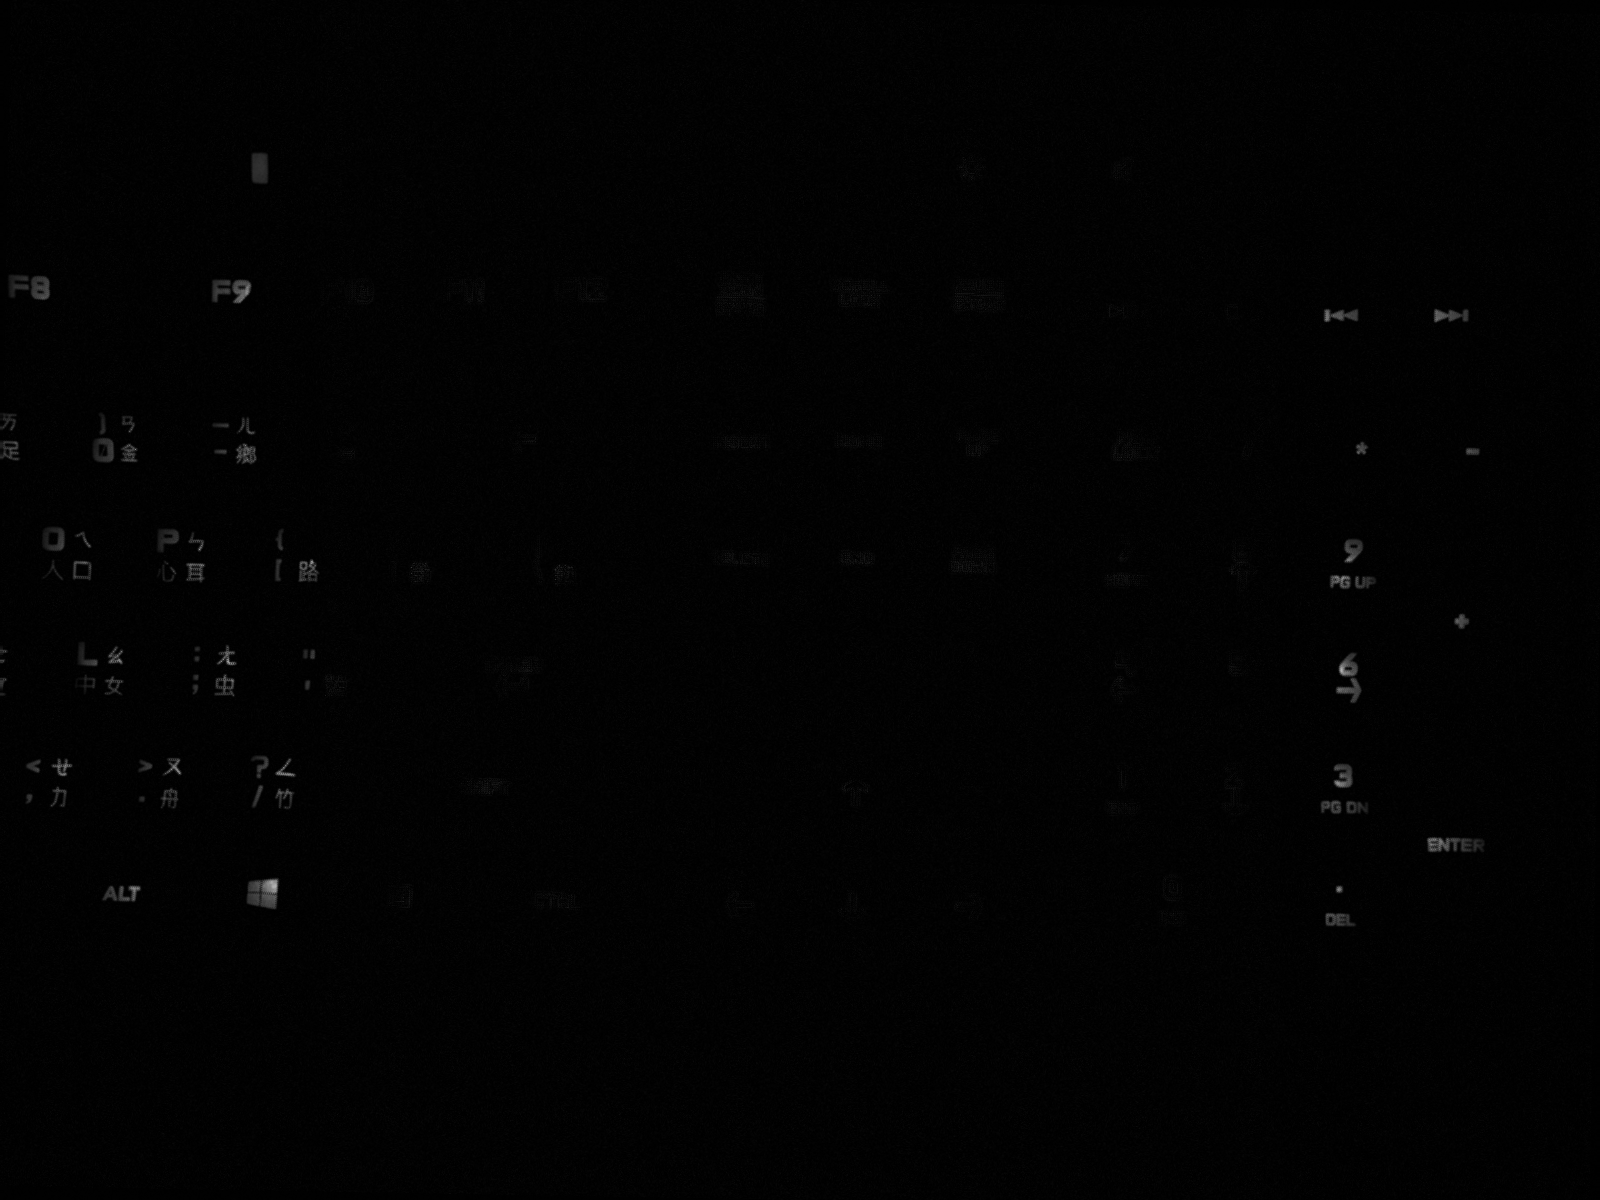
\includegraphics[width=\linewidth]{simulation/normal/akaze_absdiff.png}
			\caption{Absolute Difference Results}
			\label{fig:siftAbsDifference}
		\end{figure}



	\subsection{Unexpected Rotate}
		In this section, we'll rotate the sample image from 1 to 10 degree and 15 degree and 20 degree then observe the difference between each feature detector.
	\subsection{Unexpected Translation}
		In this section, we'll move the sample image from left to right by 30, 50, 100, 200 pixels then observe the difference between each feature detector.
	\subsection{LED failure}
		In this section, we'll mask out the sample image by deferent percentages then observe the difference between each feature detector.
		The following images were results by mask out the sample image by 20\%, 40\%, 60\%, 80\%, 85\%, 90\% and 95\%.
	\subsection{Noise of Camera}
		In this section, we'll add the salt \& pepper noise with different level to the sample image, then observe the difference between each feature detector.

\section{Comparison between each methods}
	% add execiution time compare chart here
	\subsection{Simple Blob Detector}
		\subsubsection{Introduction}
			The blob feature detector is an simple approach for feature point detection. We choose the centroid of each selected blob as the feature point. Matching feature points with nearest neighborhood. 
			Since we have a fixture that can guarantee the keyboard does not have shift or rotation more then a certain amount, we can assume that the feature point matched is the nearest one.
		\subsubsection{Performance}
			% $$\textrm{Add time data}$$
		\subsubsection{Pros \& Cons}
			This method has lowest robustness in experiment, but fastest in execution.

	\subsection{SIFT}
		\subsubsection{Introduction}
		SIFT feature is proposed by Lowe \cite{lowe2004distinctive} et al., having the state of the art robustness in most scenarios \cite{karami2017image}, but slower than any other methods on execution.
		\subsubsection{Performance}
			% $$\textrm{Add time data}$$
		\subsubsection{Pros \& Cons}
	
	\subsection{SURF}
		\subsubsection{Introduction}
		SURF is a upgrade version based on SIFT, witch is designed to solve the speed issue of SIFT. 
		And in the scenario of this thesis, this method meets the requirement on the stability without wasting too much time on calculation.
		\subsubsection{Performance}
			% $$\textrm{Add time data}$$
		\subsubsection{Pros \& Cons}

	\subsection{ORB}
		\subsubsection{Introduction}
		ORB is a
		\subsubsection{Performance}
			% $$\textrm{Add time data}$$
		\subsubsection{Pros \& Cons}

	\subsection{AKAZE}
		\subsubsection{Introduction}
		AKAZE is a
		\subsubsection{Performance}
			% $$\textrm{Add time data}$$
		\subsubsection{Pros \& Cons}